% This file contains CHAPTER SIX

\chapter{Explicit Formulas for Genus 3 Balanced Arithmetic}\label{cha:g3} In
this chapter, derivations of explicit formulas for genus 3 hyperelliptic curves
given by a split model are described. 
%Tables describing explicit formulas for doubling and addition in the frequent 
%cases are presented in Appendix~\ref{app:g3SPLIT}. 
All explicit formulas presented in this chapter are
implemented in Magma along with implementations of random input testing and
automatic generation of inputs that cover every output case. Automated operation
counting and latex table generation scripts were also developed to circumvent
errors in the operation count and explicit formula presentations. All software
developed for this thesis is available at
\url{https://github.com/salindne/divisorArithmetic}. Corresponding results for
ramified models are developed by another student and will appear together with
these results in a paper to be submitted later. 

\section{Improved Genus 3 Split Model Explicit Formulas}
In this section, novel explicit formulas for addition and doubling of divisor
classes on genus 3 hyperelliptic curves represented by split models are
described. In general, the curve equation of a split model for a genus 2
hyperelliptic curve in Weierstrass form is $C: y^2 + h(x)y = f(x)$ where
$$f = f_8x^8 + f_7x^7 + f_6x^6 + f_5x^5 + f_4x^4 + f_3x^3 + f_2 x^2 + f_1x +
f_0, \s\s\s\s\s h = h_4x^4 + h_3x^3 + h_2x^2 + h_1x + h_0,$$ where $f_8$ is a
square in $k$ if char$(k) \neq 2$ and $f_8 = \beta^2 + \beta$, for some $\beta
\in k$ otherwise. The polynomial $\Vp = \Vn_4x^4 + \Vn_3x^3 + \Vn_2x^2 + \Vn_1x
+ \Vn_0$ such that $\deg(f - \Vp(\Vp + h)) \leq 3$ (see
Definition~\ref{def:vpvn}), is precomputed in Algorithm~\ref{alg:g3explSPLITpre}
along with a table of precomputations and curve coefficients. Input and output
balanced divisors are represented by 7-coordinate vectors of six field elements
and a balancing coefficient $n$ as$$ D = [u_2,u_1,u_0,v_2,v_1,v_0,n],$$
corresponding to the Balanced Mumford representation $D = [u,v,n]$ with $u = x^3
+ u_2x^2 + u_1x + u_0$ and $v = v_2x^2 + v_1x + v_0$ in negative reduced basis
(Section~\ref{sec:reduced}).  The two leading coefficients of $v$ in any reduced
basis only rely on curve parameters and therefore still only six base field
elements are required to represent a divisor class. 

In contrast to previous work designed for arithmetic in the infrastructure of a
genus 3 split model curve~\cite{rad2019jacobian}, the formulas of this work are
complete and are designed to be efficient for arithmetic in the divisor class
group (using balanced divisor representations) as opposed to the infrastructure.
The work in~\cite{Sutherland_g3_2019} does present explicit formulas for
addition and doubling in the divisor class group for genus 3 split models using
the balanced setting, but only considers frequent cases. Moreover, the frequent
case formulas in this work require considerably fewer field operations than
previous best~\cite{rad2019jacobian} and~\cite{Sutherland_g3_2019}. The
framework introduced in this work based on balanced divisor class
representations~\cite{Galbraith_balanced_2008} and the novel Balanced NUCOMP from
Section~\ref{sec:balNUCOMP} encapsulates all adjustments in special cases,
resulting in formulas that require only one inversion given any two divisor
classes as input. Applying many of the same techniques as for genus 2 curve
formulas adapted to genus 3, and introducing some novel ones, complete explicit
formulas are developed including all special cases based on
Algorithms~\ref{alg:g3balnucomp} and~\ref{alg:g3balnudupl}.

For genus 3 split models, and odd genus in general, non-trivial calls to
adjust occur as part of the frequent cases reduction process  i.e.; adjust is
always called in the frequent case. The adjustment is not auxiliary, but
replaces the final reduction step when reducing the degree of the intermediate
divisor representative from degree four to three in Cantor's algorithm. As
suggested in Section~\ref{sec:balNUCOMP}, a negative reduced basis is used to
absorb one adjustment via the continued fraction steps of Balanced NUCOMP
resulting in removing the need for any further adjustment steps in the frequent
cases. Working with a negative reduced basis also reduces the degree of the $k =
f - v(v+h)$ polynomial that arises in the computations via cancellations.


This section is structured as follows; first, assumptions about curve models
over certain fields are discussed, followed by an overview of prior work. This
is followed by a statement of the novel contributions in this work and a
description of the basic formulations for doubling and addition.
Finally, operation costs in terms of field operations, comparisons to previous
work, and empirical benchmarking results are presented.

\subsection{Curve Simplifications} 
\label{sect:g3splitcurvesimplifications}
Recall from Section~\ref{sect:splitcurvesimplifications} that isomorphic
transformations can be applied depending on the characteristic of the base field
of the hyperelliptic curve, where the possible transformation for genus 2 curve
split models were given. On genus 3 split models, the same isomorphic
transformations can be applied over fields of characteristic 2 and not equal to
2 (Section~\ref{sect:splitcurvesimplifications}). Operation counts in
Section~\ref{sec:g3splitFieldCosts} assume the following:
\begin{itemize}
\item  If char($k) \neq 2$ then $h = 0$.
\item  If char($k) = 2$ then $h_4 = 1$ and $h_3 = f_5 = f_4 = f_3 = 0$.
\end{itemize}


\subsection{Prior Work}
\label{sec:g3explSPLITPriorWork}

In~\cite{rad2019jacobian} the authors present explicit formulas for frequent
case addition, doubling and degree zero addition (referred to as baby steps) on
genus 3 split models over characteristic 2 and characteristic not equal to 2
fields. The formulas are not presented for divisor class arithmetic, but only
the related (but different) infrastructure of a genus 3 curve split model.
Similar to the work in~\cite{EricksonJacobsonStein_realg2_2011} the authors use
a slightly different definition of Mumford representation, where $u ~|~ f + hv -
v^2$ instead of $u ~|~ f - hv - v^2$ and the alternate positive reduced
normalization of the $v$ polynomial where 
\begin{align}
  u' & =  u \nonumber\\
  v' & =  \Vp + h - [(\Vp + h - v) \mod u]. 
\end{align}

In~\cite{Sutherland_g3_2019} the author presents explicit formulas for frequent
case addition and doubling, with no special cases considered, over the divisor
class group of a split model genus 3 hyperelliptic curve using balanced
divisors. The polynomial $v$ of the Mumford representation of a divisor class is
not normalized into a reduced basis, and left exactly as-is from the definition
of Mumford representation (Definition~\ref{sec:mumford}). Comparing to operation
counts of the explicit formulas in~\cite{rad2019jacobian}, frequent case
doubling requires fewer field operations, but addition requires more field
operations than~\cite{rad2019jacobian}.

\subsection{Summary of Contributions}
This work provides complete explicit formulas, in the sense that all computation
paths are explicitly computed, requiring only one inversion in all cases that
take reduced divisor class representatives as input, and output a reduced
divisor class representative. Not only is every special case explicitly
computed, this work also considerably improves the field operation counts of
divisor class operations over previous best in the frequent cases of addition
and doubling. 
%The frequent case explicit formulas are given in Appendix~\ref{app:g3SPLIT}. 
All formulas are implemented in Magma including a
testing suite to ensure their correctness (described in
Section~\ref{sec:g3numerical}). The implemented formulas and testing scripts are
available at \url{https://github.com/salindne/divisorArithmetic}.

The explicit formulas for divisor class addition and doubling are based on Balanced
NUCOMP specialized to genus 3 addition and doubling using a negative reduced
basis (see Section~\ref{sec:reduced}) that include efficient formulations of
special cases. The explicit formulation of steps in Algorithms~\ref{alg:g3balnucomp}
and~\ref{alg:g3balnudupl}, coupled with certain explicit techniques produce the
fastest explicit formulas for frequent case addition and doubling to date. As
explained in Section~\ref{sec:comparisons}, a negative reduced basis
normalization for $v$ is beneficial to a NUCOMP based algorithm and is used in the
explicit formulas in contrast to the positive reduced basis used for genus 2
arithmetic.

A summary of the novel techniques that differ from previous work for genus 3
split model explicit formulas goes as follows:
\begin{enumerate}[label=T\arabic*] \setcounter{enumi}{9}
\item \label{tq:10} Use specialized genus 3 versions of Balanced NUCOMP and
NUDUPL Algorithms~\ref{alg:g3balnucomp} and~\ref{alg:g3balnudupl} as the basis
for all explicit formulas. Using the specialized Balanced NUCOMP variants
greatly reduces the field operation counts in the frequent cases when compared
to previous methods. For special cases, using Balanced NUCOMP instead of
Balanced ADD Algorithm~\ref{alg:impbaladd}  avoids either a second inversion or
pushes weighted values from the composition step to the adjustment step with
Montgomery's inversion trick, resulting in a significant reduction in the number
of field operations. Applying Balanced NUCOMP to degree 0 additions results in
similar formulations as Balanced Adjust Algorithm~\ref{alg:impbaladjustn}, but
this work improves on previous best with Technique~\ref{tq:11}.
\item \label{tq:11} Apply an alternate computation of the output $k$ polynomial
in all doubling and many addition algorithms with input divisor degrees of 2 or
less as described in Section~\ref{sec:alternatek}.
\item \label{tq:12} Include explicit one-inversion formulas for all special
cases with $\gcd (u_1,u_2,v_1 + v_2 + h) \not = 1$  based on
Algorithms~\ref{alg:g3balnucomp} and~\ref{alg:g3balnudupl}, producing much more
efficient formulas when compared to adaptations of previous
suggestions~\cite{EricksonJacobsonStein_realg2_2011} to genus 3.
\item \label{tq:13} Use a system of equations for $s=s_2x^2 + s_1x + s_0$,
similar to~\ref{tq:1}, but instead of solving for $s$, compute the required
inverted polynomial $q$ with weight resultant $d$ from the system as described
in Section~\ref{sec:alternateharley}. Then compute $ds = q(v_1 - v_2)
\pmod{u_2}$ applying Karatsuba multiplication (Section~\ref{sec:karatsubamul})
twice instead of a Toom style multiplication as done
in~\cite{Sutherland_g3_2019}. The net difference in operation counts for this
portion of the algorithms is 5 fewer field additions and two fewer field divisions by
2, but requires one more field multiplication when compared to~\cite{Sutherland_g3_2019}.
\end{enumerate}

Recall that the threshold for trading field multiplications for field additions
is capped at 1 multiplication for 3 additions through out (see
Section~\ref{sec:trades}.)


\subsubsection{Special Cases}
Implementations of frequent case arithmetic include explicit handling of special
cases as they come up naturally in the computations via Technique~\ref{tq:12}.
All computation paths through special cases in the formulas require only one
inversion and are based on Algorithm~\ref{alg:g3balnucomp}. Suggestions from
previous work~\cite{EricksonJacobsonStein_realg2_2011} adapted to the genus 3
split model setting, (based on the ramified model suggestions
of~\cite{Lange_explicit_2005}), for handling these cases produced far more
cumbersome explicit formulas compared to using the specialization of Balanced
NUCOMP to genus 3. The relative reduction in finite field operations can be
attributed to applying continued fraction steps from Balanced NUCOMP for
adjustment computations and the omission of invoking algorithms for lower-degree
divisor classes with weighted inputs.

The basic formulation of the frequent cases Degree 3 Addition and Doubling
algorithms are presented as Algorithms~\ref{alg:g3explSPLIT3ADD}
and~\ref{alg:g3explSPLIT3DBL} with  $v$ in negative reduced basis as input. Note
that in frequent cases, $n$ remains unchanged ($n = 0$). Several new arithmetic
cases over the divisor class group of a split model curve are presented that
were not considered in previous works. These special cases can be invoked based
on the degree and balancing coefficient $n$ of both input divisors as described
in Section~\ref{sec:comparisons}. There are four degree 0 divisors possible,
$n=0,1,2,3$, of which only one (when $n=2$) is the divisor class group's neutral
element. Degree 0 divisor doubling, and degree 0 with degree 0 addition are
completely precomputed and discussed in the next section.

\subsection{Precomputations}\label{sec:g3precompute}
Similar to the genus 2 split model setting, there is a need to compute and store
the coefficients of $\Vn$ along with curve constants, and the extra complexity
of split model arithmetic admits many curve constant computations including
degree 0 compositions completely dependent on curve constant computations. A
precomputation table is used to omit computing the same values multiple times.

\begin{algorithm}[htbp]
\caption{Precomputation\label{alg:g3explSPLITpre}}
\begin{algorithmic} [1]
\Require $h = h_4x^4 + h_3x^3 + h_2x^2 + h_1x + h_0$,
\Statex \hspace{23pt}$f = f_8x^8 + f_7x^7 + f_6x^6 + f_5x^5 + f_4x^4 + f_3x^3 + f_2x^2 + f_1x + f_0$.
\algrule
\State $\Vp_4$ is a solution to the quadratic equation $(\Vp_4)^2  + h_4\Vp_4 = f_8$.
\State $\Vn_4 = -\Vp_4 - h_4, \s\s\s c_4 = -\Vn_4 + \Vp_4, \s\s\s c_6 =1/c_4$.
\State $\Vp_3 = c_6(f_7 - \Vp_4h_3), \s\s\s \Vn_3 = -\Vp_3 - h_3$.
\State $\Vp_2 = c_6(f_6 - \Vp_4h_2 + \Vp_3\Vn_3), \s\s\s \Vn_2 = -\Vp_2 - h_2, \s\s\s c_2 = -\Vn_2 + \Vp_2$.
\State $\Vp_1 = c_6(f_5 - \Vp_4h_1 + \Vp_3\Vn_2 + \Vp_2\Vn_3), \s\s\s \Vn_1 = -\Vp_1 - h_1, \s\s\s c_1 = -\Vn_1 + \Vp_1$.
\State $c_3 = -\Vn_3 + \Vp_3, \s\s\s c_2 = -\Vn_2 + \Vp_2, \s\s\s c_1 = -\Vn_1 + \Vp_1, \s\s\s c_{10} = \Vp_2\Vn_2$.
\State $\Vp_0 = c_6(f_4 - \Vp_4h_0 + \Vp_3\Vn_1 + c_{10} + \Vp_1\Vn_3), \s\s\s \Vn_0 = -\Vp_0 - h_0$.
\State $c_0 = -\Vn_0 + \Vp_0, \s\s\s c_5 = c_4 + c_2, \s\s\s c_7 = c_1c_6, \s\s\s c_8 = c_2c_6, \s\s\s c_9 = c_3c_6$.
\State $\dn_5 = f_3 - h_0\Vn_3, \s\s\s \dn_4 = \dn_5 - h_1\Vn_2, \s\s\s \dn_3 = \dn_4 + c_2\Vn_1$.
\State $\dn_0 = f_2 - h_0\Vn_2, \s\s\s \dn_2 = \dn_0 + \Vn_1\Vp_1, \s\s\s \dn_1 = f_1 - h_0\Vn_1$.
\State $\dn_6 = \dn_1c_6, \s\s\s \dn_7 = \dn_2c_6, \s\s\s \dn_8 = \dn_3c_6, \s\s\s \dn_9 = \dn_4c_6, \s\s\s \dn_{10} = \dn_0c_6$.
\State $d_5 = f_3 - h_0\Vp_3, \s\s\s d_4 = d_5 - h_1\Vp_2, \s\s\s d_3 = d_4 + c_2\Vp_1$.
\State $d_0 = f_2 - h_0\Vp_2, \s\s\s d_2 = d_0 + \Vp_1\Vn_1, \s\s\s d_1 = f_1 - h_0\Vp_1$.
\State $d_6 = d_1c_6, \s\s\s d_7 = d_2c_6, \s\s\s d_8 = d_3c_6, \s\s\s d_9 = d_4c_6, \s\s\s d_{10} = d_0c_6$.
\State Compute $u = u_3x^3 + u_2x^2 + u_1x + u_0 = (f - \Vn(\Vn +  h) \s\s\s$ (made monic).
\State Compute $b = b_2x^2 + b_1x + b_0 = \Vn - (\Vn - \Vp) \pmod{u}$.
\State Compute $u' = u'_3x^3 + u'_2x^2 + u'_1x + u'_0 = (f - b(b +  h) \s\s\s$ (made monic).
\State Compute $b' = b'_2x^2 + b'_1x + b'_0 = \Vn - (-\Vp - b) \pmod{u'}$.
\State \Return [[$f_0,f_1,f_2,f_3,f_4,f_5,f_6,f_7,f_8$],\s[$h_0,h_1,h_2,h_3,h_4$],\s[$\Vp_0,\Vp_1,\Vp_2,\Vp_3,\Vp_4$],
\Statex \hspace{37pt} \s[$\Vn_0,\Vn_1,\Vn_2,\Vn_3,\Vn_4$],\s[$c_0,c_1,c_2,c_3,c_4,c_5,c_6,c_7,c_8,c_9,c_{10}$], 
\Statex \hspace{37pt} \s[$d_0,d_1,d_2,d_3,d_4,d_5,d_6,d_7,d_8,d_9,d_{10}$],\s[$\dn_0,\dn_1,\dn_2,\dn_3,\dn_4,\dn_5,\dn_6,\dn_7,\dn_8,\dn_9,\dn_{10}$],
\Statex \hspace{37pt} \s[$u_0,u_1,u_2,u_3,n,b_0,b_1,b_2$],\s[$u'_0,u'_1,u'_2,u'_3,n',b'_0,b'_1,b'_2$]]
\end{algorithmic}
\end{algorithm}

As stated above, in order to explicitly compute complete addition and doubling,
precomputed results for addition and doubling of divisors $[1,\Vn,0], [1,\Vn,1]$
and $[1,\Vn,3]$ are required. Depending on the hyperelliptic polynomials $f$ and
$h$, the output divisor from composing those divisor classes may be degree 3,2,
1, or 0. The computation of all possible cases is considered in the
precomputation table. For genus 3 split models, it is beneficial to store both
$\Vp = \Vp_4x^4 + \Vp_3x^3 + \Vp_2x^2 + \Vp_1x + \Vp_0$ and  $\Vn = \Vn_4x^4 +
\Vn_3x^3 + \Vn_2x^2 + \Vn_1x + \Vn_0$ as $\Vn$ is often used because of the
negative reduced basis. First, $\Vp$ is computed as described in
Definition~\ref{def:vpvn}, and then $\Vn = - \Vp - h$. Given $f$ and $h$, $\Vp$
can be computed explicitly, where the leading coefficient of $\Vp$, $\Vp_4$, is
set to be a solution to the quadratic equation $\Vp_4(\Vp_4 + h_4) = f_8$. The
precomputed $c_i$ correspond to coefficients of $c = 2\Vp + h$ and convenient
precomputations using coefficients of $c$. The $d_i$ are used throughout the
explicit formulas for positive reduced basis and the $\dn_i$ are used in
negative reduced basis. The coefficients of the polynomials $u$ and $v$ and
balancing coefficient $n$ correspond to the output after adjusting input
$[1,\Vn,-1]$, the $u'$ and $v'$ and balancing coefficient $n'$ to the output
after twice adjusting input $[1,\Vn,-2]$. The polynomials $u, \s \Vn$ and
balancing coefficient $n=0$ are re-used as the output of adjusting input
$[1,\Vn,4]$. The balancing coefficients are computed according to Steps~20,23,27
of Algorithm~\ref{alg:g3balnucomp}.

\subsection{Explicit Doubling}\label{sec:g3SPLITDBL}
In this section, complete divisor class doubling is described and the basic
formulations of the corresponding explicit formulas are provided. Doubling
Algorithm~\ref{alg:g3balnudupl} is further specialized into different cases
depending on the input divisor class degree and balancing coefficient. Any
explicit techniques used are discussed in each case. 

The complete doubling algorithm should test the degree of the input divisor in
order of statistical frequency and choose the appropriate algorithm depending on
the input balancing coefficient $n_1$. The six doubling formulas used for
complete doubling are:
\begin{itemize}
    \item Degree 3 doubling
    \item Degree 2 doubling
    \item Degree 2 doubling with two up adjustments
    \item Degree 1 doubling
    \item Degree 1 doubling with down adjustment
    \item Degree 1 doubling with two up adjustments. 
\end{itemize}  
Only precomputed values are required for degree zero doubling, and
precomputations from Algorithm~\ref{alg:g3explSPLITpre} may be used. In the
frequent cases, the output balancing coefficient $n$ is always zero, and any
special cases, $n$ is computed via Steps~5,19,23--24,31--32 of
Algorithm~\ref{alg:g3balnudupl}. Basic formulations of the algorithms required
for complete doubling, organized by the degree of the input divisor, are
described in the following.

\subsubsection{Balancing Coefficient}\label{sec:g3expldbl} 

Let $[u_1,v_1,n_1]$ be an input reduced divisor class representative. Let $S$ be
the greatest common divisor of $u_1$ and $2v_1 + h$ and $s$ be the
polynomial computed by Step~8 in Doubling Algorithm~\ref{alg:g3balnudupl}.
There are 3 main cases:\begin{itemize}
    \item [1.] If no reduction or adjustment is required as checked by Step~14
    of Doubling Algorithm~\ref{alg:g3balnudupl} , then $n_n = 2n_1 + \deg(S) -
    2$ by Step~5 of Doubling Algorithm~\ref{alg:g3balnudupl}.
    \item [2.] If $\deg(s) < 2 $, the NUCOMP continued fraction loop is not
    entered, but at least one reduction or adjustment step is required. There
    are two sub-cases, if $v_1$ is normalized with a positive reduced basis then
    $n_n = 2n_1 + \deg(S) - 2 + 2\deg(u_1) - 4$ by Step~18 of Doubling
    Algorithm~\ref{alg:g3balnudupl}. Otherwise for $v_1$ normalized with a
    negative reduced basis, $n_n = 2n_1 + \deg(S) - 2 + \deg(u_1) - \deg(s)$ by
    Step~24 unless $\deg(u_1s) < 4$, then $n_n = 2n_1 + \deg(S) - 2 + 4 -
    \deg(u_n)$ where $n_n \geq 0$. Finally, if $n_n < 0$ in the previous case, a
    final adjustment up is required and  one more computation for the balancing
    coefficient is required where $n_n = n_n + 4 - \deg(u_n)$ by Step~25 of
    Doubling Algorithm~\ref{alg:g3balnudupl}.
    \item [3.] If $\deg(s) = 2$, the NUCOMP continued fraction loop is entered
    for one iteration, resulting in $n_n = 2n_1 + \deg(S) - 2 + \deg(u_1) -
    \deg(r)$ with $r$ computed by Step~27 of Doubling
    Algorithm~\ref{alg:g3balnudupl}, unless $\deg(z) < 4$ for $z$ computed by
    Step~30 of Doubling Algorithm~\ref{alg:g3balnudupl}, in which case $n_n = 2n_1 +
    \deg(S) - 2 + \deg(u_1) - \deg(s) + 4 - \deg(u_n)$.
\end{itemize}

\subsubsection{Genus 3 Split Model Degree 3 Doubling}
Let $[u_1,v_1,n_1]$ be the input reduced divisor class representative with $u_1 = x^3 +
u_{12}x^2 + u_{11}x + u_{10}$, $v_1 = \Vn_4x^4 + \Vn_3x^3 + v_{12}x^2 + v_{11}x
+ v_{10}$ and $n_1 = 0$. Similar to genus 2 split model doubling
Algorithm~\ref{alg:g2balnudupl}, Steps~1-2 of Doubling
Algorithm~\ref{alg:g3balnudupl} are always skipped. Steps~3--8 in
Algorithm~\ref{alg:g3balnudupl} are specialized to degree 3 doubling by
computing the resultant $d = \mathrm{Res}(u_1,2v_1+h)$ instead of $S =
\mathrm{XGCD}(u_1,2v_1 + h)$ in Step~4 of Algorithm~\ref{alg:g3balnudupl}, where
$d=0$ implies $S \neq 1$. 

To compute a degree 3 double, first create the system of equations required for the
alternate computation of the $s$ polynomial in genus 3
(Section~\ref{sec:alternateharley}). As described in
Section~\ref{sec:alternateharley} only the coefficients $m_1,m_4,m_7$ and the
determinant $d = \mathrm{Res}(u_1,2v_1+h)$ are computed where $m_1,m_4,m_7$
correspond to $t = m_7x^2 + m_4x + m_1 = d/(2v_1 + h) \pmod{u_1}$. The resultant
$d$ is then immediately checked to be zero for special cases as soon as possible
in order to minimize unnecessary computations.


The computation of the $k$ polynomial in Step~3 of
Algorithm~\ref{alg:g3balnudupl} is postponed until after the computation of $d$,
and instead $d$ is immediately checked for special cases. If $d \neq 0$, then in
contrast to the genus 2 setting, the coefficients of $s$ are not solved for
directly and instead $s = kt \pmod{u_1}$ is computed in Step~8. The computation
of Steps~25--33 of Doubling Algorithm~\ref{alg:g3balnudupl} follows. If $d = 0$,
then Steps~7--24 are performed instead depending on $\deg(u_1)$ and $\deg(s)$, as
described in Subroutine~\ref{sub:g3explSPLIT3DBLd}. 

The basic formulation for degree 3 doubling is described in
Algorithm~\ref{alg:g3explSPLIT3DBL}. An explanation of how each step in
Algorithm~\ref{alg:g3explSPLIT3DBL} is converted to an explicit formula follows.
In Step~1, the polynomial representation \thickmuskip=3mu $$k'_2x^2 + k'_1x + k'_0 = (\vt_2x^2 +
\vt_1x + \vt_0)(s_2x^2 + s_1x + s_0) - (s_2\vt_2x + \vt_2s_1 + s_2(\vt_1 -
u_{12}\vt_2))(x^3 + u_{12}x^2 + u_{11}x + u_{10})$$ \thickmuskip=5mu is used to set up a system
of equations linear in the coefficients of $s$ where
$$s = s_2x^2 + s_1x + s_0 = (k'_2x^2 + k'_1x + k'_0)/(\vt_2x^2 + \vt_1x + \vt_0)
\pmod{x^3 + u_{12}x^2 + u_{11}x + u_{10}},$$ and $\vt = 2v_1 + h \pmod{x^3 +
u_{12}x^2 + u_{11}x + u_{10}}$. By equating coefficients of the polynomials in
the above identity, the following linear system of equations given by the 3 by 3
matrix $T$ arises: $$ \left(
\begin{array}{ccc} 
 t_1 = \vt_0 & t_2 = -u_{10}\vt_2        & t_3 = -u_{10}(\vt_1 - u_{12}\vt_2)  \\
 t_4 = \vt_1 & t_5 = \vt_0 - u_{11}\vt_2 & t_6 = -u_{10}\vt_2 - u_{11}(\vt_1 - u_{12}\vt_2)  \\
 t_7 = \vt_2 & t_8 = \vt_1 - u_{12}\vt_2 & t_9 = \vt_0 - u_{11}\vt_2 - u_{12}(\vt_1 - u_{12}\vt_2)  
\end{array} \right) \cdot 
\left( \begin{array}{c}
s_0  \\
s_1   \\
s_2   \end{array} \right) = 
\left( \begin{array}{c}
k_0  \\
k_1   \\
k_2   \end{array} \right).$$ 

\begin{algorithm}
\caption{Genus 3 Split Model Degree 3 Doubling\label{alg:g3explSPLIT3DBL}}
\begin{algorithmic} [1]
\Require $[D_1]= [u_1, v_1,0]$ \smallskip
\Ensure $[u_n,v_n,n_n] = 2[D_1]$
\algrule
\State Compute matrix coefficients $t_i$ representing $s(h + 2v_1)\equiv k \pmod{u_1}$ as the 3x3 linear system $ \left[
\begin{smallmatrix} t_1 & t_2 & t_3\\ t_4 & t_5 & t_6\\ t_7 &t_8 & t_9 \end{smallmatrix}\right] \left[
\begin{smallmatrix} s_0\\ s_1 \\s_2 \end{smallmatrix} \right] = \left[ \begin{smallmatrix} k_0\\ k_1\\ k_2 \end{smallmatrix} \right]$.
\State Compute coefficients $m_1 = t_5t_9, \s m_4 = t_6t_7 - t_4t_9, \s m_7 = t_4t_8 - t_5-t_7$ of the inverse of the matrix and let $t = m_7x^2 + m_4x + m_1$.
\State $d = t_1m_1 + t_2m_4 + t_3m_7$.
\If{$d = 0$} 
\State Go to Degree 3 Doubling ($d=0$) Subroutine~\ref{sub:g3explSPLIT3DBLd}.
\EndIf
\State $k' = (f - v_1(v_1 + h))/u_1 \pmod{u_1}$.
\State $s' = ds = s_2'x^2 + s_1'x + s_0' =  k't \pmod{u_1}$.
\If{$s_2' = 0$} 
\State Go to Degree 3 Doubling ($s_2=0$) Subroutine~\ref{sub:g3explSPLIT3DBLs2}.
\EndIf
\State Compute monic quotient $q'= x + s'_2(q_0/q_1) = x + q'_0$ of $u_1/s'$ with $1/q_1 = s_2$. 
\State Compute remainder $r' = s'_2dr = r'_1x + r'_0$ of $u_1/s'$.
\If{$r'_1$ is 0} 
\State Go to Degree 3 Doubling ($r'_1=0$) Subroutine~\ref{sub:g3explSPLIT3DBLr1}.
\EndIf
\State Compute values $q_1/r_1, r_1/q_1, q_0/q_1, r_0/q_1, q_0/r_1, r_0/r_1$.
\State $M_2' = (r(2v_1 + h) + qk)/u_1 \s\s\s $(exact division, made monic).
\State $u_n = r^2/(c_4r_1q_1) - qM_2'/q_1.$
\State $z = (u_1r - u_n(c_4r_1q_1))/q \s\s\s$ (exact division).
\State $v_n = \Vn - [(\Vn - z + v_1 + h) \pmod{u_n}]$.
\State \Return $[u_n,v_n,0]$.
\end{algorithmic}
\end{algorithm}

The resulting explicit formula for Step~1 is
\begin{align*}
    T_0  &= u_{12}c_4,\\
    T_1  &= c_3 - T_0,\\
    v_{n_0} &= -v_{10} - h_0,\\
    v_{n_1} &= -v_{11} - h_1,\\    
    v_{n_2} &= -v_{12} - h_2,\\
    \vh_1 &= v_{11} - v_{n_1},\\
    \vh_2 &= v_{12} - v_{n_2},\\
    t_1 &= v_{10} - v_{n_0} + u_{10}T_1,\\
    t_4 &= \vh_1 + u_{10}c_4 + u_{11}T_1,\\
    t_7 &= \vh_2 + u_{11}c_4 + u_{12}T_1,\\
    t_2 &= -u_{10}t_7,\\
    t_5 &= t_1 - u_{11}t_7,\\
    t_8 &= t_4 - u_{12}t_7,\\
    t_3 &= -u_{10}t_8,\\
    t_6 &= t_2 - u_{11}t_8,\\
    t_9 &= t_5 - u_{12}t_8.
\end{align*}
In Steps~2--3, the inverse of $T$ from Step~1 is computed omitting divisions by $\det(T)$, yielding
$$ \det(T)T^{-1} = M = \left( \begin{array}{ccc}
m_1 = t_5t_9 - t_8t_6 & m_2 = t_3t_8 - t_2t_9 & m_3 = t_2t_6 - t_3t_5  \\
m_4 = t_6t_7 - t_4t_9 & m_5 = t_1t_9 - t_3t_7 & m_6 = t_3t_4 - t_1t_6  \\
m_7 = t_4t_8 - t_5t_7 & m_8 = t_2t_7 - t_1t_8 & m_9 = t_1t_5 - t_2t_4
\end{array} \right).$$ 
Only the terms $m_1,m_4,m_7$ are required to compute the polynomial inversion of
$\vt$ modulo $u_1$ where $$ t = m_7x^2 + m_4x + m_1 = \frac{d}{\vt}
\pmod{u_1}$$ without the field inversion to divide by $d$. The computation of $d = \det(T)$ is
chosen to reuse the same $m_i$. The resulting explicit formula for Steps~2--3 is
\begin{align*}
    m_1 &= t_5t_9 - t_6t_8,\\
    m_4 &= t_6t_7 - t_4t_9,\\
    m_7 &= t_4t_8 - t_5t_7,\\
    d   &= t_1m_1 + t_2m_4 + t_3m_7. 
\end{align*} 
The value $d = 0$ is then checked for special cases as soon as possible in order
to minimize unnecessary computations. 

If $d \neq 0$, in Step~6  $k' = (f - v_1(v_1 + h))/u_1 \pmod{u_1}$ is computed
by an exact division, and school book modular reduction of a degree 3 polynomial
by a monic degree 3 modulus. Coefficients $k_i$ of $k$ without the modular
reduction are saved. The explicit formula for Step~6 is \newpage
\begin{align*}
    t_1  &= v_{11} - \Vn_1,\\
    t_2  &= v_{12} - \Vn_2,\\
    k_3  &= c_4t_2,\\
    t_{10} &= u_{12}k_3,\\
    k_2  &= c_3t_2 + c_4t_1 - t_{10},\\
    k_2' &= k_2 - t_{10},\\
    t_{11} &= u_{11}k_3,\\
    k_1  &= c_4(v_{10} - \Vn_0) + c_3t_1 + v_{21}v_{n_2} - c_{10} - u_{12}k_2 - t_{11},\\
    k_1' &= k_1 - t_{11},\\
    t_{12} &= u_{10}k_3,\\
    k_0'  &= d_{n_5} + c_3v_{10} - h_2v_{11} - v_{12}\vh_1 - u_{11}k_2 - u_{12}k_1 - t_{12} - t_{12}.
\end{align*}

In Step~7, $s' = k't \pmod{u_1}$ is computed by applying Karatsuba
multiplication (see Section~\ref{sec:karatsubamul}), and Karatsuba modular
reduction (see Section~\ref{sec:karatsubared}) of a degree 4 polynomial and
monic degree 3 modulus. The explicit formula for Step~7 is
\begin{align*}
    t_0 &= k_0'm_1,\\
    t_1 &= k_1'm_4,\\
    t_2 &= k_2'm_7,\\
    t_3 &= (m_4 + m_7)(k_1' + k_2') - t_2 - t_1 - u_{12}t_2,\\
    t_4 &= u_{11}t_2,\\
    t_5 &= t_4 - t_1,\\
    s_0' &= t_0 - u_{10}t_3,\\
    s_1' &= (m_1 + m_4)(k_0' + k_1') - s_0' - (u_{10} + u_{11})(t_2 + t_3) + t_5,\\
    s_2' &= (m_1 + m_7)(k_0' + k_2') - t_0 - t_2 - t_5 - u_{12}t_3.
\end{align*}

Rather than directly computing the polynomials $q = q_1x + q_0$ and $r = r_1x +
r_0$, monic $q$ with weight $s'_2$ and weighted $r$ with weight $s'_2d$ are
computed as $q'$ and $r'$ in Steps~10--11 and note that $q_1 = 1/s_2 = d/s_2'$. The value
$r'_1=0$ is immediately checked after creation to minimize unnecessary
computations.  The resulting explicit formula for Steps~10--11 (with the actual
values given in brackets) is
\begin{align*} 
    & t_6 = s_2^{\prime 2},                                   && (s_2^2d^2) \\
    & t_7 = ds_2',                                            && (s_2d^2) \\ 
    & q'_0 = u_{12}s_2' - s_1',                                && ((q_0/q_1)s_2d) \\
    & r'_1 = t_6u_{11} - s_0's_2' - s_1'q_0',                   && ((r_1/q_1)s_2d^2)\\
    & r'_0 = t_6u_{10} - s_0'q_0',              && ((r_0/q_1)  s_2  d^2)
\end{align*}
If $r'_1 \neq 0$, all necessary ratios of the coefficients of $q$ and $r$ that
arise in Steps~15--18 for computing $M'_2,u_n,v_n$ are computed beforehand in
Step~14. A description of how these values are applied is given respectively in
each corresponding step. The explicit formula for Step~14 (with the actual
values given in brackets) is
\begin{align*}
   & w_3 = (t_7r'_1)^{-1},                    && ((q_1/r_1)  (1/(s_2^2  d^4)))\\
   & w_4 = w_3r'_1,                           && (1/(s_2  d^2)) \\ 
   & w_5 = w_4d,                             && (1/(s_2  d)) \\
   & w_6 = r_1'w_5^2c_4,                      && (r_1  c_4) \\
   & q_{r_{11}} = w_3t_7^2,                  && (q_1/r_1) \\
   & r_{q_{11}} = r_1'w_4,                    && (r_1/q_1) \\
   & q_{q_{01}} = q_0'w_5,                    && (q_0/q_1) \\
   & r_{q_{01}} = r'_0w_4,                    && (r_0/q_1) \\
   & q_{r_{01}} = q_{q_{01}}q_{r_{11}},      && (q_0/r_1) \\
   & r_{r_{01}} = r_{q_{01}}q_{r_{11}}.      && (r_0/r_1)
\end{align*}

In Step~15, $M_2' = M_2/(c_4r_1) = (r(2v_1 + h) + qk)/((c_4r_1)u_1)$ the
negative of $M_2$ monic is computed instead of $M_2$, with $c_6 = 1/c_4$. The
polynomial $M_2 = (r(2v_1 + h) + qk)/u_1$ is directly computed and then
symbolically multiplied by $1/(r_1c_4)$ where all terms in the equation for each
coefficient $M'_{21}$ and $M'_{20}$ that have divisions by $q_1$ or $r_1$ are
replaced with the precomputed ratios from Step~14. Any terms that require a
division by $c_4$ are grouped together and multiplied by $c_6$. The explicit
formula for Step~15 is  
\begin{align*} 
    & M'_{21} = c_6(c_3 - q_{r_{11}}k_3) + r_{r_{01}} - u_{12}    \\
    & M'_{20} = c_6(r_{r_{01}}c_3 - 2v_{12} - h_2 - q_{r_{11}}k_2 - q_{r_{01}}k_3) - u_{11} - u_{12}M'_{21}.
\end{align*}
In Step~16, the output polynomial $$u_n = r^2 - qM_2 = r^2/(c_4r_1q_1) +
(qM'_2)/q_1$$ is computed using the same approach as in Step~15. The explicit
formula for Step~16 is: 
\begin{align*} 
    & u_{n_2} = c_6r_{q_{11}} + M'_{21} + q_{q_{01}}          \\
    & u_{n_1} = c_6r_{q_{01}}M'_{20} + q_{q_{01}}M'_{21}    \\
    & u_{n_0} = c_6r_{q_{01}}r_{r_{01}} + q_{q_{01}}M'_{20}.
\end{align*}
The original leading coefficient of $u_n$ is $c_4r_1q_1$. Since $u_n$ is required to
be monic, the computation of $z = (ru_1 - u_n)/q$ in Step~17 must be adjusted to
$z = (ru_1 - u_n(c_4r_1q_1))/q$. The exact polynomial division by $q = q_1x +
q_0$ introduces divisions in the coefficients of $z$ where the precomputed
ratios from Step~14 are used instead. Steps~17 and~18 are combined as
$$v_n = \Vn - [(\Vn + v_1 + h - z) \pmod{u}],$$ using a Karatsuba modular
reduction (see Section~\ref{sec:karatsubared}) to perform the modular reduction.
The explicit formula for Steps~17--18 is
\begin{align*} 
    & t_3 = c_3 + r_{q_{11}} - u_{n_2}c_4,                   \\
    & t_2 = r_{q_{11}}(u_{n_2} - q_{q_{01}}) + r_{q_{01}} - w_6,   \\
    & t_1 = r_{q_{11}}u_{11} + r_{q_{01}}  u_{12} - w_6u_{n_2} - q_{q_{01}}t_2, \\
    & t_5 = u_{n_0}t_3,       \\
    & t_4 = u_{n_1}c_4,       \\
    & v_2 = -v_{12} - h_2 + t_2 - t_4 - u_{n_2}t_3,       \\
    & v_1 = -v_{11} - h_1 + t_1 - (u_{n_0} + u_{n_1})(c_4 + t_3) + t_4 + t_5,   \\
    & v_0 = -v_{10} - h_0 + r_{q_{11}}  u_{n_0} - w_6u_{n_1} - q_{q_{01}}t_1 - t_5.
\end{align*}

Basic formulations of the special output cases $s_2' = 0$ and $r_1 = 0$ are
given in Subroutines~\ref{sub:g3explSPLIT3DBLs2}
and~\ref{sub:g3explSPLIT3DBLr1}. There are two types of special output cases,
$\deg(s') < 2$ and $\deg(s) = 2$ but $\deg(r) < 1$. If $\deg(s') < 2$, then the
computation of $q,r$ is omitted and the output is computed similarly to degree 2
doubling Algorithm~\ref{alg:explSPLIT2DBL}.  In the case that $\deg(s') = 2$ but
$\deg(r) < 1$, then $\deg(z) < 4$ and lower degree output divisors using same
approach as the frequent case are computed with output $n_n$ computed as
described in Section~\ref{sec:g3expldbl}.  

\begin{subroutine}[htbp]
\caption{Genus 3 Split Model Degree 3 Doubling ($s_2' = 0$)\label{sub:g3explSPLIT3DBLs2}}
\begin{algorithmic} [1]
\If{$s_1'$ is 0}
    \If{$s_0'$ is 0} \Return $[1,\Vp,2]$.
    \Else
        \State Compute $1/(s_0)$ and $s = s_0$.
        \State $M_2 = (s(2v_1 + h) - k)/u_1 \s\s\s $(exact division).
        \State $u_n = s^2 + M_2, \s\s\s $ (made monic).
        \State $v_n = \Vn - (\Vn + su_1 + v_1 + h) \pmod{u_n}$.
        \State \Return $[u_n,v_n,1]$
    \EndIf
\EndIf
\If{Degree 4 term $M_{24}$ of $s(2v_1 + h) - k$ is 0}
    \If{Degree 3 term $M_{23}$ of $s(2v_1 +h) - k$ is 0} \Return $[1,\Vn,0]$
    \Else
        \State Compute $1/M_{24}$ and $s = s_0$.
        \State $M_2 = (s(2v_1 + h) - k)/u_1 \s\s\s $(exact division).
        \State $u_n = s^2 + M_2, \s\s\s $ (made monic).
        \State $v_n = \Vn - (\Vn + su_1 - v_1 - h) \pmod{u_n}$.
        \State \Return $[u_n,v_n,0]$
    \EndIf
\EndIf
\State Compute $1/M_{25}$ degree 5 term of $s(2v_1 + h) - k$ and $s = s_1x + s_0$.
\State $M_2 = (s(2v_1 + h) - k)/u_1 \s\s\s $(exact division).
\State $u_n = s^2 + M_2, \s\s\s $ (made monic).
\State $v_n = \Vn - (\Vn + su_1 - v_1 - h) \pmod{u_n}$.
\State \Return $[u_n,v_n,0]$.
\end{algorithmic}
\end{subroutine}

\begin{subroutine}[htbp]
\caption{Genus 3 Split Model Degree 3 Doubling ($r_1 = 0$)\label{sub:g3explSPLIT3DBLr1}}
\begin{algorithmic} [1]
    \If{$r_0$ is 0} 
    \State $u_n = -q^2k/u_1, \s\s\s$ (exact division, made monic)
    \State $v_n = \Vn - (\Vn - v_1 - h) \pmod{u_n}$.
    \State \Return $[u_n,v_n,2]$.
\Else
    \If{Degree 4 term $M_{24}$ of $r(2v_1 + h) - qk$ is 0}
        \If{Degree 3 term $M_{23}$ of $r(2v_1 + h) - qk$ is 0} \Return $[1,\Vn,3]$
        \Else
            \State Compute $1/M_{24}$ and $r_0$.
            \State $M_2 = (r(2v_1 + h) + qk)/u_1 \s\s\s $(exact division).
            \State $u_n = r^2 - qM_2, \s\s\s $ (made monic).
            \State $z = (u_1r - u_n)/q \s\s\s$ (exact division).
            \State $v_n = \Vn - [(\Vn - z + v_1 + h) \pmod{u_n}]$.
            \State \Return $[u_n,v_n,2]$
        \EndIf
    \EndIf
    \State Compute $1/q_1$, $q_0/q_1$ and $r_0/q_1$.
    \State $M_2 = (r(2v_1 + h) + qk)/u_1 \s\s\s $(exact division).
    \State $u_n = r^2 - qM_2, \s\s\s $ (made monic).
    \State $z = (u_1r - u_n(c_4r_0 + q_1k_3))/q \s\s\s$ (exact division).
    \State $v_n = \Vn - [(\Vn - z + v_1 + h) \pmod{u_n}]$.
    \State \Return $[u_n,v_n,1]$
\EndIf
\end{algorithmic}
\end{subroutine}

The basic formulation of the special case $d = 0$ is described in
Subroutine~\ref{sub:g3explSPLIT3DBLd}. This case implies that
$\gcd{(h + 2v_1, u_1)}$ has either degree 1, 2 or 3. Similarly to genus 2 split
model doubling (Algorithm~\ref{sub:explSPLIT2DBLd}), the common factor is
removed from $u_1$ via an exact division (Section~\ref{sec:exactdiv}), and
$s,u_,v_n$ are then computed accordingly depending on the degree.
The output balancing coefficient $n_n$ is computed as described in
Section~\ref{sec:g3expldbl}.

\begin{subroutine}[htbp]
\caption{Genus 3 Split Model Degree 3 Doubling ($d = 0$) \label{sub:g3explSPLIT3DBLd}}
\begin{algorithmic} [1]
\If{$m_7$ is 0}
    \If{$t_7$ is 0} \hspace{1pt} \Return $[1,\Vn,1]$.
    \Else \hspace{2pt} $d_w =  (h + 2v_1) \pmod{u_1} = t_7x^2 + t_4x + t_1.$
        \State $b_1 = 1/$lcf$(d_w)$ and $d_w$ made monic.
        \State $k = (f - v_1(v_1 + h))/u_1$.
        \State $u_1 = u_1/d_w$.
        \State $s = b_1k \pmod{u_1}$.
        \State $u_n = u_1^2$, $v_n = \Vn - (\Vn - v_1 - u_1s) \pmod{u_n}$.
        \State \Return $[u_n,v_n,0]$
    \EndIf
\Else \hspace{2pt} $m_8 = t_2t_7 - t_1t_8$. 
    \State $S = -m_7x + m_8$.
    \State $u'_1 = u_1/S = u'_{11}x + u'_{10}$ where $u'_{11}$ has weight $m_7$ and $u'_{10}$ weight $m_7^2$.        
    \State Compute $m_i$ in system of equations for $su_1\equiv \vt \pmod{u_2}$ as $ \bigl[ \begin{smallmatrix} m_1 & m_2\\ m_3 & m_4\end{smallmatrix}\bigr] \bigl[ \begin{smallmatrix} s_0\\ s_1 \end{smallmatrix} \bigr ] = \bigl[ \begin{smallmatrix}\vt_0 \\  \vt_1\end{smallmatrix} \bigr ]$,
    \Statex \hspace{18pt}  where $\vt = \vt_1x + \vt_0 = (2v_1 + h) \pmod{u'_1}$.
    \State $d_2 = m_1m_4 - m_2m_3$.  
    \State $k = (f - v_1(v_1 + h))/u'_1)$.
    \State Solve for $s_1(d_2/m_7), s_0(d_2)$ using $m_i$ and Cramer's rule, omitting the inversion of $d_2$.
    \If{$s_1(d_2/m_7)$ is 0} 
        \If{$s_0(d_2)$ is 0} 
            \If{$k_3 = 0$} \hspace{2pt} $u_n = -k/u_1, \s\s\s$ (made monic).
                \State $v_n = \Vn - (\Vn + v_1 + h) \pmod{u_n}$.
                \State \Return $[u_n,v_n,2]$
            \Else \hspace{2pt} $u_n = -k/u_1, \s\s\s$ (made monic).
                \State $v_n = \Vn - (\Vn + v_1 + h) \pmod{u_n}$.
                \State \Return $[u_n,v_n,1]$
            \EndIf
        \Else
            \If{Degree 4 term $M_{24}$ of $s(2v_1 + h) - k$ is 0}
                \If{Degree 3 term $M_{23}$ of $s(2v_1 +h) - k$ is 0} \Return $[1,\Vn,3]$
                \Else \hspace{2pt} Compute $1/M_{24}$, and unweighted $u_1$.
                    \State $M_2 = (s(2v_1 + h) - k)/u'_1 \s\s\s $(exact division).
                    \State $u_n = s^2 + M_2, \s\s\s $ (made monic).
                    \State $v_n = \Vn - (\Vn + su_1 - v_1 - h) \pmod{u_n}$.
                    \State \Return $[u_n,v_n,2]$
                \EndIf
            \EndIf
            \State Compute $1/M_{24}$, $s = s_0$ and unweighted $u_1$.
            \State $M_2 = (s(2v_1 + h) - k)/u'_1 \s\s\s $(exact division).
            \State $u_n = s^2 + M_2, \s\s\s $ (made monic).
            \State $v_n = \Vn - (\Vn + su_1 - v_1 - h) \pmod{u_n}$.
            \State \Return $[u_n,v_n,1]$
        \EndIf
    \EndIf
    \State Compute $s = s_1x + s_0$ and unweighted $u_1$ and $k$.
    \State $M_2 = (s(2v_1 + h) - k)/u'_1 \s\s\s $(exact division).
    \State $u_n = s^2 + M_2, \s\s\s $ (made monic).
    \State $v_n = \Vn - (\Vn + su_1 - v_1 - h) \pmod{u_n}$.
    \State \Return $[u_n,v_n,0]$.
\EndIf
\end{algorithmic}
\end{subroutine}


\newpage
\subsubsection{Genus 3 Split Model Degree 2 Doubling}
Let $[u_1,v_1,n_1]$ be the input reduced divisor class representative with $u_1
= x^2 + u_{11}x + u_{10}$, $v_1 = \Vn_4x^4 + \Vn_3x^3 + \Vn_2x^2 + v_{11}x +
v_{10}$ and $n_1 = 0$ or $n_1 = 1$. There are two degree 2 doubling algorithms
required for complete divisor class arithmetic; degree 2 doubling, and degree 2
doubling with two up adjusts. The balancing coefficient $n = 2n_1 - 2$ is -2 or
0, depending on whether $n_1$ is 0 or 1 respectively. The degree of the divisor
after degree 2 doubling is 4 (where $4 = g + 1$), so an adjustment is required
for a final reduction step. 

If $n_1 = 1$ then a down adjustment is applied as part of the reduction by
normalizing $v_1$ in positive reduced basis before any other computations. If
$n_1=0$, then an up adjustment is applied as the reduction bringing the
balancing coefficient to -1 and a second up adjustment is required for $n$ to be
in range. The composition and first adjustment steps are combined via continued
fraction steps of Doubling Algorithm~\ref{alg:g3balnudupl} as described
in~\ref{tq:10}, and the second up adjustment for degree 2 doubling with two up
adjusts is applied as described in Steps~21--23 of
Algorithm~\ref{alg:g3balnudupl} using Montgomery's inversion trick
(Section~\ref{sec:montgomery}). The basic formulation for degree 2 doubling is
described in Algorithm~\ref{alg:g3explSPLIT2DBL}. An explanation of how each
step in Algorithm~\ref{alg:g3explSPLIT2DBL} is converted to an explicit formula
is given in the following.

\begin{algorithm}[htbp]
\caption{Genus 3 Split Model Degree 2 Doubling\label{alg:g3explSPLIT2DBL}}
\begin{algorithmic} [1]
\Require $[D_1]= [u_1, v_1,1]$ \smallskip
\Ensure $[u_n,v_n,n_n] = 2[D_1]$
\algrule
\State $v_1 = \Vp - [(\Vp - v_1) \pmod{u_1}].$
\State Compute $t_i$ in system for $s(h + 2v_1)\equiv k \pmod{u_1}$ as $ \bigl[
\begin{smallmatrix} m_1 & m_2\\ m_3 & m_4\end{smallmatrix}\bigr] \bigl[
\begin{smallmatrix} s_0\\ s_1 \end{smallmatrix} \bigr ] = \bigl[ \begin{smallmatrix}k_0
\\  k_1\end{smallmatrix} \bigr ]$, where $(h + 2v_1) \pmod{u_1} = d_w = -m_3x + m_4.$
\State $d = m_1m_4 - m_2m_3$.
\If{$d = 0$}
    \If{$m_3$ is 0} \hspace{1pt} \Return $[1,\Vp,2]$.
    \Else
        \State $k = (f - v_1(v_1 + h))/u_1$.
        \State $b_1 = 1/$lcf$(d_w)$ and $d_w$ made monic.
        \State $u_1 = u_1/d_w$.
        \State $s = b_1k \pmod{u_1}$.
        \State $u_n = u_1^2$.
        \State $v_n = \Vp - (\Vp - v_1 - u_1s) \pmod{u_n}$.
        \State \Return $[u_n,v_n,1]$.
    \EndIf
\EndIf
\State $z = z_3x^3 + z_2x^2 + z_1x + z_0 = (f - v_1(v_1 + h))/(c_4u_1) \pmod{u_1}.$
\State Solve for $s_1' = ds_1, s_0' = ds_0$ using $m_i$ and Cramer's rule, omitting the inversion of $d$.
\If{$s_1' = 0$} 
    \If{$s_0' = 0$} 
        \If{$z_3 = 0$} \Return $[1,\Vn,0]$.
        \Else
            \State Compute $1/z_3$.
            \State $u_n = z/u_1 \s\s\s $(exact division, made monic).
            \State $v_n = \Vn - (\Vn - v_1 - h) \pmod{u_n}$.
            \State \Return $[u_n,v_n,0]$
        \EndIf
    \Else \hspace{4pt}
        \State Compute $1/s_0$ and $s= s_0$.
        \State $M_2 = (s(2v_1 + h)/c_4 - z)/u_1 \s\s\s $(exact division).
        \State $u_n = s^2 + M_2, \s\s\s $ (made monic).
        \State $v_n = \Vn - (\Vn + su_1 + v_1 + h) \pmod{u_n}$.
        \State \Return $[u_n,v_n,0]$
    \EndIf
\EndIf
\State Compute $1/(s_1)$ and $s = s_1x + s_0$.
\State $M_2 = (s(2v_1 + h)/c_4 - z)/u_1 \s\s\s $(exact division).
\State $u_n = s^2 + M_2, \s\s\s $ (made monic).
\State $v_n = \Vn - (\Vn + su_1 + v_1 + h) \pmod{u_n}$.
\State \Return $[u_n,v_n,0]$.
\end{algorithmic}
\end{algorithm}
The formulation of degree 2 doubling in the balanced setting over genus 3 split
models, including the special case where $d=0$, is similar to degree 2
doubling over genus 2 split models (Algorithm~\ref{alg:explSPLIT2DBL}). Both compute
the composition related to a degree 4 intermediate divisor class representative,
but in the genus 2 case, there is a reduction to a degree 2 or less divisor
class representative, and in genus 3 the reduction results in a degree 3 or less
divisor class representative via an adjustment step. Adjustment steps only have
one possibility for a special output case, instead of two as in
Algorithm~\ref{alg:explSPLIT2DBL}. The alternate computation of $k$
(Technique~\ref{tq:8}) from Algorithm~\ref{alg:explSPLIT2DBL} is adapted to the
genus 3 setting where $z = k/c_4 = (f - v_1(v_1 + h))/u_1c_4$ is computed
instead (Technique~\ref{tq:11}).

The basic formulation for degree 2 doubling with two up adjustments is described in
Algorithm~\ref{alg:g3explSPLIT2DBL2UP}. An explanation of how each step in
Algorithm~\ref{alg:g3explSPLIT2DBL2UP} is converted to an explicit formula is given
in the following.

\begin{algorithm}[htbp]
\caption{Genus 3 Split Model Degree 2 Doubling with two Up Adjusts\label{alg:g3explSPLIT2DBL2UP}}
\begin{algorithmic} [1]
\Require $[D_1]= [u_1, v_1,0]$ \smallskip
\Ensure $[u_n,v_n,n_n] = 2[D_1]$
\algrule
\State $v_1 = \Vp - [(\Vp - v_1) \pmod{u_1}].$
\State Compute $t_i$ in system for $s(h + 2v_1)\equiv k \pmod{u_1}$ as $ \bigl[
\begin{smallmatrix} m_1 & m_2\\ m_3 & m_4\end{smallmatrix}\bigr] \bigl[
\begin{smallmatrix} s_0\\ s_1 \end{smallmatrix} \bigr ] = \bigl[ \begin{smallmatrix}k_0
\\  k_1\end{smallmatrix} \bigr ]$, where $(h + 2v_1) \pmod{u_1} = d_w = -m_3x + m_4.$
\State $d = m_1m_4 - m_2m_3$.
\If{$d = 0$}
    \State Go to Genus 3 Split Model Degree 2 Doubling with 2 Up Adjusts ($d=0$) Subroutine~\ref{sub:g3explSPLIT2DBL2UPd}.
\EndIf
\State $k = k_3x^3 + k_2x^2 + k_1x + k_0 = (f - v_1(v_1 + h))/u_1 \pmod{u_1}.$
\State Solve for $s_1(d), s_0(d)$ using $m_i$ and Cramer's rule, omitting the inversion of $d$.
\If{$s_1' = 0$} 
    \If{$s_0' = 0$} 
        \If{$k_3 = 0$} \Return $[1,\Vn,2]$.
        \Else \hspace{3pt}Compute $1/k_3$.
            \State $u_n = k/u_1 \s\s\s $(exact division, made monic).
            \State $v_n = \Vn - (\Vn - v_1 - h) \pmod{u_n}$.
            \State \Return $[u_n,v_n,1]$
        \EndIf
    \Else \hspace{3pt} Compute $1/s_0$ and $s= s_0$.
        \State $M_2 = (s(2v_1 + h)/c_4 - z)/u_1 \s\s\s $(exact division).
        \State $u_n = s^2 + M_2, \s\s\s $ (made monic).
        \State $v_n = \Vn - (\Vn + su_1 + v_1 + h) \pmod{u_n}$.
        \State \Return $[u_n,v_n,0]$
    \EndIf
\EndIf
\State $W = -s_1(d)d, \s\s\s W_2 = W^2$.
\State $M_2 = (s(2v_1 + h)- k)/u_1, \s$ with weight $W$.
\State $u' = s^2 + M_2, \s $ with weight $W$.
\State $v' = \Vn - (\Vn + su_1 + v_1 + h) \pmod{u'}$, with weight $W_2$.
\State $w = w_6x^6 + w_5x^5 + w_4x^4 + w_3x^3 + w_2x^2 +w_1x + w_0 = (f - v'(v' + h))/c_4$, weighted.
\State Compute $1/W$, $1/W_2$ and unweighted $u',v'$
\State $u_n = w/u' \s\s\s$ (exact division, made monic).
\State $v_n = \Vn - (\Vn + v' + h) \pmod{u_n}$.
\State $n_n = 3 - \deg(u_n)$.
\State \Return $[u_n, v_n,n_n]$.
\end{algorithmic}
\end{algorithm}
Degree 2 doubling with two adjusts is similar to degree 2 doubling, but does not
normalize $v_1$ into positive reduced basis, and requires one more adjustment
step at the end. The inversion in the degree 2 doubling portion is omitted using
Montgomery's inversion trick (see Section~\ref{sec:montgomery}), and is instead
computed in the final adjustment. Computing $z = k/c_4$ instead of $k$ by
Technique~\ref{tq:11} does not benefit any operation that requires 2 up
adjustments and is omitted. 

The basic formulation for degree 2 doubling with two adjusts is described in
Subroutine~\ref{sub:g3explSPLIT2DBL2UPd}. An explanation of how each step in
Subroutine~\ref{sub:g3explSPLIT2DBL2UPd} is converted to an explicit formula is
given in the following.

\begin{algorithm}[htbp]
\caption{Genus 3 Split Model Degree 2 Doubling with two Up Adjusts ($d = 0$)\label{sub:g3explSPLIT2DBL2UPd}}
\begin{algorithmic} [1]
\If{$m_3$ is 0} \hspace{1pt} \Return $[1,\Vp,0]$.
\EndIf
\State $k = (f - v_1(v_1 + h))/u_1$.
\State $u_1(-m_3) = u_1/d_w$, with weight $-m_3$.
\State $s = k \pmod{u_1(-m_3)}$, with weight $M_3 = (-m_3)^3$.
\State $k = kdw$, with weight $M_4 = m_3^4$.
\If{Degree 4 term $M_{24}$ of $s(2v_1 + h) - k$ is 0}
    \If{Degree 3 term $M_{23}$ of $s(2v_1 +h) - k$ is 0} 
        \If{Degree 2 term $M_{22}$ of $s(2v_1 +h) - k$ is 0} \Return $[1,\Vn,3]$
        \Else \hspace{3pt} Compute $1/m_3$, $1/M_{22}$ and $s = s_0$.
            \State $M_2 = (s(2v_1 + h) - k)/u_1 \s\s\s $(exact division).
            \State $u_n = s^2 + M_2, \s\s\s $ (made monic).
            \State $v_n = \Vn - (\Vn + su_1 - v_1 - h) \pmod{u_n}$.
            \State \Return $[u_n,v_n,2]$
        \EndIf
    \Else \hspace{3pt} Compute $1/m_3$, $1/M_{23}$ and $s = s_0$.
        \State $M_2 = (s(2v_1 + h) - k)/u_1 \s\s\s $(exact division).
        \State $u_n = s^2 + M_2, \s\s\s $ (made monic).
        \State $v_n = \Vn - (\Vn + su_1 - v_1 - h) \pmod{u_n}$.
        \State \Return $[u_n,v_n,1]$
    \EndIf
\EndIf
\State Compute $1/m_3$, $1/M_{24}$ and $s = s_0$.
\State $M_2 = (s(2v_1 + h) - k)/u_1 \s\s\s $(exact division).
\State $u_n = s^2 + M_2, \s\s\s $ (made monic).
\State $v_n = \Vn - (\Vn + su_1 - v_1 - h) \pmod{u_n}$.
\State \Return $[u_n,v_n,1]$
\end{algorithmic}
\end{algorithm}
For $d=0$, a second up adjustment is not required in any cases, as the degree of
the common divisor $\gcd(u_1,2v_1 + h)$ is added to the balancing coefficient
$n_n$ as described in Section~\ref{sec:g3expldbl}, resulting in a similar
approach to Degree 2 doubling Algorithm~\ref{alg:explSPLIT1DBLUP} computing the
single up adjustment on a degree 1 doubling. Lower degree output divisor class
representatives are compute based on cancellations in the coefficients of $M_2$.

\subsubsection{Degree 1 Doubling}
Let $[u_1,v_1,n_1]$ be the input reduced divisor class representative with $u_1 = x +
u_{10}$, $v_1 = \Vn_4x^4 + \Vn_3x^3 + \Vn_2x^2 + \Vn_1x + v_{10}$ and $n_1 = 0$,
$n_1 = 1$ or $n_1 = 2$.  There are three degree 1 doubling algorithms required
for complete divisor class arithmetic; degree 1 doubling, degree 1 doubling with
down adjust and degree 1 doubling with two up adjusts. Depending on the input
balancing coefficient, if $n_1$ is 0,1 or 2, the resulting $n = 2n_1 - 2$ value
is -2, 0 or 2 respectively. The degree of the divisor after degree 1 doubling is
2, and so the output balancing coefficient range is $n \in [0,1]$. If $n_1 = 0$
two up adjustments are required to produce a reduced divisor class
representative, if $n_1 = 1$ then no adjustments are required, and if $n_1 = 2$
then one down adjustment is required. The formulation of degree one doubling
Algorithm~\ref{alg:g3explSPLIT1DBL} follows Doubling
Algorithm~\ref{alg:g3balnudupl} closely. The basic formulation for degree 1
doubling is described in Algorithm~\ref{alg:g3explSPLIT1DBL}. \vspace{10pt}
\begin{algorithm}[htbp]
\caption{Genus 3 Split Model Degree 1 Doubling\label{alg:g3explSPLIT1DBL}}
\begin{algorithmic} [1]
\Require $[D_1] = [u_1,v_1,1]$.  \smallskip
\Ensure $[u_n,v_n,n_n] = 2[D_1]$.
\algrule
\State $d = (h + 2v_1)/c_4 \pmod{u_1}$.
\If{$d = 0$} \Return $[1,\Vn,1]$.
\EndIf
\State $z = (f - v_1(v_1 + h))/(c_4u_1)$.
\State $s_0 = z/d \pmod{u_1}. \s\s$ (note that $1/d = b_1 \pmod{u_1}$ in Alg~\ref{alg:g3balnudupl})
\State $u_n = u_1^2$.
\State $v_n = \Vn - (\Vn -s_0u_1 - v_1)  \pmod{u_n}.$
\State \Return $[u_n,v_n,0]$.
\end{algorithmic}
\end{algorithm}
Degree 1 Doubling Algorithm~\ref{alg:g3explSPLIT1DBL} is similar to 
genus 2 Degree 1 Addition ($d=0$) Subroutine~\ref{sub:explSPLIT1ADDd}, where the
balancing coefficient $n_n$ is computed as described in
Section~\ref{sec:g3expldbl}. 

For degree 1 double with down adjust, $v_1$ is
first normalized into positive reduced basis accommodating a down adjustment as
described in Section~\ref{sec:comparisons}. The composition and adjustment steps
are combined via Doubling Algorithm~\ref{alg:g3balnudupl} as described
in~\ref{tq:10}. If $d$ is 0, then the degree of $S$ from line~4 of
Algorithm~\ref{alg:g3balnudupl} is one, resulting in a degree 0 divisor output
where the balancing coefficient is computed as $n_n = 2n_1 + \deg(S) - 2 = 3$ based
on the input balancing coefficient $n_1 = 2$ (see Section~\ref{sec:g3expldbl}).
Special output cases corresponding to the degree of $s(2v + h)/c_4 - z$ after
the adjustment step are accounted for. The basic formulation for Degree 1
Doubling with down Adjust is described by
Algorithm~\ref{alg:g3explSPLIT1DBLDWN}. 
\begin{algorithm}[htbp]
\caption{Genus 3 Split Model Degree 1 Doubling with Down Adjust \label{alg:g3explSPLIT1DBLDWN}}
\begin{algorithmic} [1]
\Require $[D_1] = [u_1,v_1,2]$.  \smallskip
\Ensure $[u_n,v_n,n_n] = 2[D_1]$.
\algrule
\State
\State $d = (h + 2v_1) \pmod{u_1}$.
\If{$d = 0$} \Return $[1,\Vn,3]$.
\EndIf
\State $z = (f - v_1(v_1 + h))/(c_4u_1)$.
\State $s_0' = ds_0 = c_4z \pmod{u_1} \s\s$ with weight $d$.
\If{$s_0' = 0$}
    \State $u_n = -z/u_n \s\s\s$ (exact division, made monic).
    \State $v_n = \Vn - (\Vn - v_1)  \pmod{u_n}.$
    \State \Return $[u_n,v_n,0]$
\EndIf
\State Compute $1/s_0$ and $s = s_0$.
\State $M_2 = (s(2v_1 + h)/c_4 - z)/u_n \s\s\s $ (exact division, made monic).
\State $u_n = s_0^2 + M_2$.
\State $v = \Vn - (\Vn - s_0u_1 - v_1)  \pmod{u_n}.$
\State \Return $[u_n,v,0]$.
\end{algorithmic}
\end{algorithm}
Degree one doubling with down adjustment Algorithm~\ref{alg:g3explSPLIT1DBLDWN}
is similar to genus 2 Degree 1 Doubling with Down Adjust
Algorithm~\ref{alg:explSPLIT1DBLDWN}, with the addition of normalizing $v_1$
into positive reduced basis at the beginning. The balancing coefficient $n_n$ is
computed as described in Section~\ref{sec:g3expldbl}.

For degree 1 double with two up adjusts, the composition and first adjustment
step are combined via continued
fraction steps of Doubling Algorithm~\ref{alg:g3balnudupl} as described
in~\ref{tq:10}, and the second up adjustment is applied as described in
Steps~21--23 of Algorithm~\ref{alg:g3balnudupl} using Montgomery's inversion
trick (Section~\ref{sec:montgomery}). If $d = 0$, then the degree of $S$ from
line~4 of Algorithm~\ref{alg:g3balnudupl} is one, resulting in a degree 0
divisor output, where the balancing coefficient is computed as $n = 2n_1 + \deg(S)
- 2 = -1$ based on the input balancing coefficient $n_1 = 0$ (see
Section~\ref{sec:g3expldbl}). A precomputed adjustment of $[1,\Vn,-1]$ is
returned (see Section~\ref{sec:g3precompute}). Both special output cases
corresponding to the degree of $s(2v_1 + h) - k$ after continued fraction steps,
and the degree of $f - v(v +h)$ in the extra adjustment step are accounted for.
Technique~\ref{tq:11} is not applied in this case due to the use of Montgomery's
trick. The basic formulation for degree 1 doubling with two up adjustments is
described by Algorithm~\ref{alg:g3explSPLIT1DBLUP2}.

\begin{algorithm}[htbp]
\caption{Genus 3 Split Model Degree 1 Doubling with Two Up Adjusts \label{alg:g3explSPLIT1DBLUP2}}
\begin{algorithmic} [1]
\Require $[D_1] = [u_1,v_1,0]$.  \smallskip
\Ensure $[u_n,v_n,n_n] = 2[D_1]$.
\algrule
\State
\State $d = (h + 2v_1) \pmod{u_1}$.
\If{$d = 0$} \Return Precomputed up adjustment of $[1,\Vn,-1]$.
\EndIf
\State $k = (f - v_1(v_1 + h))/u_1$.
\State $s_0' = ds_0 = k \pmod{u_1} \s\s$ with weight $d$.
\If{$s_0' = 0$}
    \State $u_n = -k/u_n \s\s\s$ (exact division, made monic).
    \State $v_n = \Vn - (\Vn - v_1)  \pmod{u_n}.$
    \State $n_n = 3 - \deg(k)$
    \State \Return $[u_n,v_n,n_n]$
\EndIf
\State $W = s_0'd, \s\s\s W_2 = W^2$.
\State $M_2 = (s_0'(2v_1 + h)- k)/u_1, \s$ with weight $W$.
\State $u' = (s_0')^2 + M_2, \s $ with weight $W$.
\State $v' = \Vn - (\Vn + s_0'u_1 + v_1 + h) \pmod{u'}$, with weight $W_2$.
\State $w = w_6x^6 + w_5x^5 + w_4x^4 + w_3x^3 + w_2x^2 +w_1x + w_0 = (f - v(v + h))/c_4$, weighted.
\State Compute $1/W$, $1/W_2$ and unweighted $u',v'$
\State $u_n = w/u' \s\s\s$ (exact division, made monic).
\State $v_n = \Vn - (\Vn + v + h) \pmod{u_n}$.
\State $n_n = 3 - \deg(u_n)$.
\State \Return $[u_n,v_n,n_n]$.
\end{algorithmic}
\end{algorithm}
Degree 1 doubling with two up adjustments Algorithm~\ref{alg:g3explSPLIT1DBLUP2}
is similar to genus 2 Degree 1 Doubling with Up Adjust
Algorithm~\ref{alg:explSPLIT1DBLUP}, for the composition and first adjustment
portion. Instead of inverting at the end of the first adjustment, a second
adjustment is computed with weighted polynomials $u',v'$ similar to Degree 2
Doubling with 2 up adjustments Algorithm~\ref{alg:g3explSPLIT2DBL2UP}. The
balancing coefficient $n_n$ is computed as described in
Section~\ref{sec:g3expldbl}.


\subsection{Explicit Addition}\label{sec:g3SPLITADD}
In this section, complete divisor addition and the basic formulations of all the
corresponding explicit formulas are described. Addition 
Algorithm~\ref{alg:g3balnucomp} is further specialized into different cases
depending on the input divisor class degree and balancing coefficient.

The complete addition algorithm should test the degree of the input divisors in
order of statistical frequency and choose the appropriate algorithm depending on
the input balancing coefficients $n_1$ and $n_2$. 26 addition formulas are
required for complete addition:
\begin{itemize}
    \item[-] degree 3 addition,
    \item[-] degree 2 and 3 addition,
    \item[-] degree 2 and 3 addition with up adjustment,
    \item[-] degree 2 addition,
    \item[-] degree 2 addition with up adjustment,
    \item[-] degree 2 addition with two up adjustments, 
    \item[-] degree 1 and 3 addition,  
    \item[-] degree 1 and 3 addition with up adjustment,
    \item[-] degree 1 and 3 addition with two up adjustments,  
    \item[-] degree 1 and 2 addition,
    \item[-] degree 1 and 2 addition with down adjustment,   
    \item[-] degree 1 and 2 addition with up adjustment,
    \item[-] degree 1 and 2 addition with two up adjustments, 
    \item[-] degree 1 addition,
    \item[-] degree 1 addition with down adjustment,
    \item[-] degree 1 addition with up adjustment,
    \item[-] degree 1 addition with two up adjustments, 
    \item[-] degree 0 and 3 addition with down adjustment,
    \item[-] degree 0 and 3 addition with up adjustment,
    \item[-] degree 0 and 3 addition with two up adjustments,  
    \item[-] degree 0 and 2 addition with down adjustment,
    \item[-] degree 0 and 2 addition with up adjustment,
    \item[-] degree 0 and 2 addition with two up adjustments, 
    \item[-] degree 0 and 1 addition with down adjustment,
    \item[-] degree 0 and 1 addition with up adjustment, 
    \item[-] degree 0 and 1 addition with two up adjustments.  
\end{itemize}
Only precomputed values are required for degree zero addition, and
precomputations from Algorithm~\ref{alg:g3explSPLITpre} may be used. In the
frequent cases, the output balancing coefficient $n$ is always zero, and any
special cases, $n$ is computed via Steps~12,20--23,27,33--34, of
Algorithm~\ref{alg:g3balnucomp}. Basic formulations of the algorithms required
in complete addition, organized by the degree of the input divisors, are
described next. 

\subsubsection{Balancing Coefficient}\label{sec:g3expladd} 

Let $[u_1,v_1,n_1]$ and $[u_2,v_2,n_2]$ be the input reduced divisor class
representatives. Let $S$ be the greatest common divisor of $u_1$, $u_2$ and $v_2
+ v_1 + h$ and $s$ be the polynomial computed by Step~9 or~11 in Addition
Algorithm~\ref{alg:g3balnucomp}. There are 3 main cases:\begin{itemize}
    \item [1.] If no reduction or adjustment is required as checked by Step~14
    of Addition Algorithm~\ref{alg:g3balnucomp} , then $n_n = n_1 + n_2 +
    \deg(S) - 2$ by Step~12 of Addition Algorithm~\ref{alg:g3balnucomp}.
    \item [2.] Otherwise, if $\deg(s) < 2 $, the NUCOMP continued fraction loop
    is not entered, but at least one reduction or adjustment is required. There
    are two sub-cases, if $v_1$ is normalized with a positive reduced basis then
    $n_n = n_1 + n_2 + \deg(S) - 2 + \deg(u_1) + \deg(u_2) - 4$ by Step~21 of
    Addition Algorithm~\ref{alg:g3balnucomp}. Otherwise for $v_1$ normalized
    with a negative reduced basis, $n_n = n_1 + n_2 + \deg(S) - 2 + \deg(u_2) -
    \deg(s)$ by Step~24 unless $\deg(u_1s) < 4$, then $n_n = n_1 + n_2 + \deg(S)
    - 2 + 4 - \deg(u_n)$ where $n_n \geq 0$. Finally, if $n_n < 0$ in the
    previous case, a final adjustment up is required and  one more computation
    for the balancing coefficient is required where $n_n = n_n + 4 - \deg(u_n)$
    by Step~28 of Addition Algorithm~\ref{alg:g3balnucomp}.
    \item [3.] If $\deg(s) = 2$, the NUCOMP continued fraction loop is entered
    for one iteration, resulting in $n_n = n_1 + n_2 + \deg(S) - 2 + \deg(u_2) -
    \deg(r)$ with $r$ computed by Step~30 of Addition
    Algorithm~\ref{alg:g3balnucomp}, unless $\deg(z) < 4$ for $z$ computed by
    Step~34 of Addition Algorithm~\ref{alg:g3balnucomp}, in which case $n_n = n_1 + n_2 +
    \deg(S) - 2 + \deg(u_2) - \deg(s) + 4 - \deg(u_n)$.
\end{itemize}


\subsubsection{Degree 3 Addition}
Let $[u_1,v_1,0]$ and $[u_2,v_2,0]$ be the input reduced divisor class
representatives with a $u_1 = x^3 + u_{12}x^2 + u_{11}x + u_{10}$, $v_1 =
\Vn_4x^4 + \Vn_3x^3 + v_{12}x^2 + v_{11}x + v_{10}$ and $u_2 = x^3 + u_{12}x^2 +
u_{21}x + u_{20}$, $v_2 = \Vn_4x^4 + \Vn_3x^3 + v_{22}x^2 + v_{21}x + v_{20}$.
Similar to genus 2 split model addition Algorithm~\ref{alg:g2balnucomp},
Steps~1-2 of Addition Algorithm~\ref{alg:g3balnucomp} are always skipped.
Steps~3--8 in Algorithm~\ref{alg:g3balnucomp} are specialized to degree 3
addition by computing the resultant $d = \mathrm{Res}(u_1,u_2)$ instead of $S =
\mathrm{XGCD}(u_1,u_2)$ in Step~4 of Algorithm~\ref{alg:g3balnucomp}, where
$d=0$ implies $S \neq 1$. 

To compute a degree 3 addition, first create the system of equations required for the
alternate computation of the $s$ polynomial in genus 3
(Section~\ref{sec:alternateharley}).  Only $m_1,m_4,m_7$ and the determinant $d$ are
computed at first where $d$ corresponds to the resultant of $u_1$ and $u_2$
and $m_1,m_4,m_7$ correspond to $t = m_7x^2 + m_4x + m_1 = d/u_1
\pmod{u_2}$. The resultant $d$ is then immediately checked to be zero for
special cases as soon as possible in order to minimize unnecessary computations.

The computation of the $k$ polynomial in Step~3 of
Algorithm~\ref{alg:g3balnucomp} is postponed until after the computation of $d$,
and instead $d$ is immediately checked for special cases. If $d \neq 0$, then in
contrast to the genus 2 setting, the coefficients of $s$ are not solved for
directly and instead $s = (v_2 - v_1)t \pmod{u_2}$ is computed in Step~11. The
computation of Steps~30--38 of Addition Algorithm~\ref{alg:g3balnucomp} follows,
where  the computation of $M_1$ and $u_n$ is combined. The basic formulation for
degree 3 addition is described in Algorithm~\ref{alg:g3explSPLIT3ADD}. An
explanation of how each step in Algorithm~\ref{alg:g3explSPLIT3ADD} is converted
to an explicit formula is given in the following.

\begin{algorithm}
\caption{Genus 3 Split Model Degree 3 Addition\label{alg:g3explSPLIT3ADD}}
\begin{algorithmic} [1]
\Require $[D_1]= [u_1, v_1,0]$, $[D_2]= [u_2, v_2,0]$, $\deg(u_1) = \deg(u_2) = 3$.
\Ensure $[u_n,v_n,n_n] = [D_1] + [D_2]$
\algrule
\State Compute matrix coefficients $t_i$ representing $su_1\equiv (v_1 - v_2) \pmod{u_2}$ as the 3x3 linear system $ \left[
\begin{smallmatrix} t_1 & t_2 & t_3\\ t_4 & t_5 & t_6\\ t_7 &t_8 & t_9 \end{smallmatrix}\right] \left[
\begin{smallmatrix} s_0\\ s_1 \\s_2 \end{smallmatrix} \right] = \left[ \begin{smallmatrix}k_0
\\  k_1 \\ k_2 \end{smallmatrix} \right]$.
\State Compute coefficients $m_1 = t_5t_9, \s m_4 = t_6t_7 - t_4t_9, \s m_7 = t_4t_8 - t_5-t_7$ of the inverse of the matrix and let $t = m_7x^2 + m_4x + m_1$.
\State $d = t_1m_1 + t_2m_4 + t_3m_7$.
\If{$d = 0$} 
\State See description below.
\EndIf
\State $\vt = \vt_2x^2 + \vt_1x + \vt_0 = v_2 - v_1$.
\State $s' = ds = s_2'x^2 + s_1'x + s_0' =  \vt t \pmod{u_2}$.
\If{$s_2'$ is 0} 
\State Go to Degree 3 Addition ($s_2=0$) Subroutine~\ref{sub:g3explSPLIT3ADDs2}.
\EndIf
\State Compute monic quotient $q'= x + s'_2(q_0/q_1) = x + q'_0$ of $u_1/s'$ with $1/q_1 = s_2$. 
\State Compute remainder $r' = s'_2dr = r'_1x + r'_0$ of $u_1/s'$.
\If{$r'_1$ is 0}
\State Go to Degree 3 Addition ($r'_1=0$) Subroutine~\ref{sub:g3explSPLIT3ADDr1}.
\EndIf
\State Compute values $q_1/r_1, r_1/q_1, q_0/q_1, r_0/q_1, q_0/r_1, r_0/r_1$.
\State $k = (f - v_1(v_1 + h)/u_1) \s\s\s $ (only degree 2 and 3 terms $k_2,k_3$).
\State $M_2' = (r(v_2 + v_1 + h) + qk)/u_2 \s\s\s $(exact division, made monic).
\State $u_n = r(q(v_2 - v_1) + u_1r)/(u_2c_4r_1q_1) - qM_2'/q_1.$
\State $z = (u_1r - u_n(c_4r_1q_1))/q \s\s\s$ (exact division).
\State $v_n = \Vn - [(\Vn - z + v_1 + h) \pmod{u_n}]$.
\State \Return $[u_n,v_n,0]$.
\end{algorithmic}
\end{algorithm} In Step~1, similar to degree 3 doubling
Algorithm~\ref{alg:g3explSPLIT3DBL}, the polynomial representation \begin{align*}
    \vt = u_1s
- (s_2x^2 + (s_2(u_{12} - u_{22}) + s_1)x &+ s_2(u_{11} - u_{21} + u_{22}(u_{12}
- u_{22})) \\
        &+ s_1(u_{12} - u_{22}))(x^3 + u_{22}x^2 + u_{21}x + u_{20})
\end{align*} for
$\vt = (v_{22} - v_{12})x^2 + (v_{21} - v_{11})x + (v_{20} - v_{10})$, $u_1 =
x^3 + u_{12}x^2 + u_{11}x + u_{10}$ and $s = s_2x^2 + s_1x + s_0$ is used to set
up a system of equations linear in the coefficients of $s$ where
$$s = s_2x^2 + s_1x + s_0 = (\vt_2x^2 + \vt_1x + \vt_0)/(x^3 + u_{12}x^2 +
u_{11}x + u_{10}) \pmod{x^3 + u_{22}x^2 + u_{21}x + u_{20}}.$$ Equating
coefficients of the polynomials in the above identity results in a 3 by 3
matrix $T$ with coefficients $t_i$. The resulting explicit formula for
Step~1 is
\begin{align*}
    t_1 &= u_{10} - u_{20},\\
    t_4 &= u_{11} - u_{21},\\
    t_7 &= u_{12} - u_{22},\\
    t_2 &= -u_{20}t_7,\\
    t_5 &= t_1 - u_{21}t_7,\\
    t_8 &= t_4 - u_{22}t_7,\\
    t_3 &= -u_{20}t_8,\\
    t_6 &= t_2 - u_{21}t_8,\\
    t_9 &= t_5 - u_{22}t_8.
\end{align*}
In Steps~2--3, the inverse of $T$ from Step~1 is computed omitting divisions by
$\det(T)$, yielding 
$$ \det(T)T^{-1} = M = \left( \begin{array}{ccc}
m_1 = t_5t_9 - t_8t_6 & m_2 = t_3t_8 - t_2t_9 & m_3 = t_2t_6 - t_3t_5  \\
m_4 = t_6t_7 - t_4t_9 & m_5 = t_1t_9 - t_3t_7 & m_6 = t_3t_4 - t_1t_6  \\
m_7 = t_4t_8 - t_5t_7 & m_8 = t_2t_7 - t_1t_8 & m_9 = t_1t_5 - t_2t_4
\end{array} \right).$$ Only the terms $m_1,m_4,m_7$ are required to compute the
polynomial inversion of $\vt$ modulo $u_1$ where $$ t = m_7x^2 + m_4x + m_1 =
\frac{d}{\vt} \pmod{u_1}$$ omitting the field inversion to divide by $d$. The
computation of $d = \det(T)$ is chosen to reuse the same $m_i$. The resulting
explicit formula for Steps~2--3 is
\begin{align*}
    m_1 &= t_5t_9 - t_6t_8,\\
    m_4 &= t_6t_7 - t_4t_9,\\
    m_7 &= t_4t_8 - t_5t_7,\\
    d   &= t_1m_1 + t_2m_4 + t_3m_7. 
\end{align*} 
The value $d = 0$ is then checked for special cases as soon as possible in order
to minimize unnecessary computations. 

If $d \neq 0$, in Step~6  $\vt = v_2 - v_1$ is computed, where the degree 3
and 4 terms cancel and no modular reduction is required. The explicit formula
for Step~6 is
\begin{align*}
    \vt_2 &= v_{22} - v_{12},\\
    \vt_1 &= v_{21} - v_{11},\\ 
    \vt_0 &= v_{20} - v_{10}.
\end{align*}
In Step~7, $s' = \vt t \pmod{u_2}$ is computed by applying Karatsuba
multiplication (see Section~\ref{sec:karatsubamul}), and Karatsuba modular
reduction (see Section~\ref{sec:karatsubared}) of a degree 4 polynomial and
monic degree 3 modulus. The explicit formula for Step~7 is
\begin{align*}
    t_0 &= \vt_0m_1,\\
    t_1 &= \vt_1m_4,\\
    t_2 &= \vt_2m_7,\\
    t_3 &= (m_4 + m_7)(\vt_1 + \vt_2) - t_2 - t_1 - u_{22}t_2,\\
    t_4 &= u_{21}t_2,\\
    t_5 &= t_4 - t_1,\\
    s_0' &= t_0 - u_{20}t_3,\\
    s_1' &= (m_1 + m_4)(\vt_0 + \vt_1) - s_0' - (u_{20} + u_{21})(t_2 + t_3) + t_5,\\
    s_2' &= (m_1 + m_7)(\vt_0 + \vt_2) - t_0 - t_2 - t_5 - u_{22}t_3.
\end{align*}

Rather than directly computing the polynomials $q = q_1x + q_0$ and $r = r_1x +
r_0$, monic $q$ with weight $s'_2$ and weighted $r$ with weight $s'_2d$ are
computed as $q'$ and $r'$ in Steps~10--11 and note that $q_1 = 1/s_2 = d/s_2'$.
The value $r'_1=0$ is immediately checked after creation to minimize unnecessary
computations. If $r'_1 \neq 0$, all necessary ratios of the coefficients of $q$
and $r$ that arise in Steps~16--19 for computing $M'_2,u_n,v_n$ are computed
beforehand in Step~14. A description of how these values are applied is given
respectively in each corresponding step. The explicit formula for Steps~10
and~14 is identical to that used in the same steps in Degree 3 Doubling
Algorithm~\ref{alg:g3explSPLIT3DBL}. 

In Step~15, only the degree 2 and 3 terms of $k = (f - v_1(v_1 + h)/u_1)$ are
computed and are similar to the computation of $k$ in degree 3 doubling
Algorithm~\ref{alg:g3explSPLIT3DBL}. The explicit formula for Step~14 is
\begin{align*}
    t_0 &= v_{12} - \Vn_2,\\
    k_3 &= c_4t_0,\\
    k_2 &= c_4(v_{11} - \Vn_1) + c_3t_0 - u_{12}k_3.
\end{align*}
In Step~16, $M_2' = M_2/(c_4r_1) = (r(2v_1 + h) + qk)/((c_4r_1)u_1)$ the
negative of $M_2$ monic is computed instead of $M_2$, with $c_6 = 1/c_4$. The
polynomial $M_2 = (r(2v_1 + h) + qk)/u_1$ is directly computed and then
symbolically multiplied by $1/(r_1c_4)$ where all terms in the equation for each
coefficient $M'_{21}$ and $M'_{20}$ that have divisions by $q_1$ or $r_1$ are
replaced with the precomputed ratios from Step~14. Any terms that require a
division by $c_4$ are grouped together and multiplied by $c_6$. The explicit
formula for Step~16 is  
\begin{align*} 
    & M'_{21} = c_6(c_3 - q_{r_{11}}k_3) + r_{r_{01}} - u_{22}    \\
    & M'_{20} = c_6(r_{r_{01}}c_3 - v_{22} - v_{12} - h_2 - q_{r_{11}}k_2 - q_{r_{01}}k_3) - u_{21} - u_{22}M'_{21}.
\end{align*}
In Step~17, the output polynomial $u_n = rM_1 - qM_2$ from
Algorithm~\ref{alg:g3balnucomp} is directly computed monic using the
computations from Step~14 as  $$r(q(v_2 - v_1) + u_1r)/(u_2c_4r_1q_1) -
qM_2'/q_1,$$ using the same approach as in Step~16. The explicit formula for
Step~15 is: 
\begin{align*} 
    & u_{n_2} = c_6r_{q_{11}} + M'_{21} + q_{q_{01}}          \\
    & u_{n_1} = c_6(r_{\vt_2 + r_{q_{11}}t_7 + r_{q_01}} + r_{q_{01}}) + M'_{20} + q_{q_{01}}M'_{21}    \\
    & u_{n_0} = c_6(r_{\vt_2r_{r_{01}} + r_{q_01}}(t_7 + r_{r_{01}})) q_{q_{01}}M'_{20}.
\end{align*}
Since $u_n$ is required to be monic, the computation of $z = (ru_1 - u_n)/q$ in
Step~17 must be adjusted to $z = (ru_1 - u_n(c_4r_1q_1))/q$. The exact
polynomial division by $q = q_1x + q_0$ introduces divisions in the coefficients
of $z$ where the precomputed ratios from Step~14 are used instead. Steps~17
and~18 are combined as $$v_n = \Vn - [(\Vn + v_1 + h - z) \pmod{u}],$$ using a
Karatsuba modular reduction (see Section~\ref{sec:karatsubared}) to perform the
modular reduction. The explicit formula for Steps~17-18 is identical to that used in the same
steps in Degree 3 Doubling Algorithm~\ref{alg:g3explSPLIT3DBL}. 

Basic formulations of the special output cases $s_2' = 0$ and $r_1 = 0$ are given
in Subroutines~\ref{sub:g3explSPLIT3ADDs2} and~\ref{sub:g3explSPLIT3ADDr1}. An
explanation of how each step in both subroutines is converted to an explicit
formula is given in the following.

\begin{subroutine}
\caption{Genus 3 Split Model Degree 3 Addition $s_2' = 0$ \label{sub:g3explSPLIT3ADDs2}}
\begin{algorithmic} [1]
\If{$s_1' = 0$}
    \If{$s_0' = 0$} \Return $[1,\Vp,2]$.
    \Else
        \State Compute $1/(s_0)$ and $s = s_0$.
        \State $(s_0(s_0u_1 + 2v_1 + h) - k)/u_2, \s\s\s$ (made monic);
        \State $v_n = \Vn - (\Vn + su_1 - v_1 - h) \pmod{u_n}$.
        \State \Return $[u_n,v_n,1]$
    \EndIf
\EndIf
\If{Degree 4 term $w_4$ of $su_1 + 2v_1 + h$ is 0}
    \If{Degree 3 term $w_3$ of $su_1 + 2v_1 + h$ is 0} \Return $[1,\Vn,0]$
    \Else
        \State Compute $1/s_1w_3$ and $s = s_1x + s_0$.
        \State Compute degree 3 term of $k = (f-v_1(v_1 = h))/u_1$.
        \State $u_n = s(su_1 + 2v_1 + h) - k)/, \s\s\s $ (made monic).
        \State $v_n = \Vn - (\Vn + su_1 - v_1 - h) \pmod{u_n}$.
        \State \Return $[u_n,v_n,0]$
    \EndIf
\EndIf
\State Compute $1/s_1w_4$ and $s = s_1x + s_0$.
\State Compute degree 3 term of $k = (f-v_1(v_1 = h))/u_1$.
\State $u_n = s(su_1 + 2v_1 + h) - k)/, \s\s\s $ (made monic).
\State $v_n = \Vn - (\Vn + su_1 - v_1 - h) \pmod{u_n}$.
\State \Return $[u_n,v_n,0]$.
\end{algorithmic}
\end{subroutine}

\begin{subroutine}
\caption{Genus 3 Split Model Degree 3 Addition $r_1 = 0$ \label{sub:g3explSPLIT3ADDr1}}
\begin{algorithmic} [1]
\State Compute degree 2 and 3 terms $k_2$ and $k_3$ of $k = (f - v_1(v_1 +h))/u_1$.
\If{$r_0$ is 0} 
    \State $M_2 = kq/u2 \s\s\s$ (exact division)
    \State $u_n = -qM_2$
    \State $v_n = \Vn - (\Vn - M_2 -v_1 - h) \pmod{u_n}$.
    \If{$k_3 = 0$} \hspace{3pt} \Return $[u_n,v_n,2]$.
    \Else \hspace{55pt} \Return $[u_n,v_n,1]$.
    \EndIf
\Else
    \If{Degree 4 term $M_{24}$ of $r(v_1 + v_2 + h) - qk$ is 0}
        \If{Degree 3 term $M_{23}$ of $r(v_1 + v_2s + h) - qk$ is 0} \Return $[1,\Vn,3]$
        \Else
            \State Compute $1/M_{23}$ and $r_0$.
            \State $M_1 = q(v_2 - v_1) + u_1r)/u_2 \s\s\s $(exact division).
            \State $M_2 = (r(2v_1 + h) + qk)/u_1 \s\s\s $(exact division).
            \State $u_n = rM_1 - qM_2, \s\s\s $ (made monic).
            \State $z = (u_1r - u_n(M_{23}))/q \s\s\s$ (exact division).
            \State $v_n = \Vn - [(\Vn - z + v_1 + h) \pmod{u_n}]$.
            \State \Return $[u_n,v_n,2]$
        \EndIf
    \EndIf
    \State Compute $1/M_{24}$ and $r_0$.
    \State $M_1 = q(v_2 - v_1) + u_1r)/u_2 \s\s\s $(exact division).
    \State $M_2 = (r(2v_1 + h) + qk)/u_1 \s\s\s $(exact division).
    \State $u_n = rM_1 - qM_2, \s\s\s $ (made monic).
    \State $z = (u_1r - u_n(M_{24}))/q \s\s\s$ (exact division).
    \State $v_n = \Vn - [(\Vn - z + v_1 + h) \pmod{u_n}]$.
    \State \Return $[u_n,v_n,1]$
\EndIf
\end{algorithmic}
\end{subroutine}
There are two types of special output cases, $\deg(s) < 2$ and $\deg(s) = 2$ but
$\deg(r) < 1$. If $\deg(s) < 2$, then the computation of $q,r$ is omitted and
the output is computed similarly to degree 2 addition
Algorithm~\ref{alg:explSPLIT2ADD}.  In the case that $\deg(s') = 2$ but $\deg(r)
< 1$, then $\deg(z) < 4$ and lower degree output divisors using same approach as
the frequent case are computed with output $n_n$ computed as described in
Section~\ref{sec:g3expladd}. 


The basic formulation of the special case $d = 0$ is omitted. The number of
special sub cases for $d=0$ grows considerably with the input degree. Instead
the following high level description is provided in which all the required
special cases can be derived easily. If $d$ is zero then $w_1 = u_1 \pmod {u_2}$
is computed for $\deg(u_2) \leq \deg(u_1)$, where the degree of $w_1$ dictates
the number of common $x$-coordinates between the two divisor class inputs. If
$w_1=0$, then there are three common point $x$-coordinates between, $u_1$ and
$u_2$, if $\deg(w_1) = 1$ then there are two common $x$-coordinates, and if
$\deg(w_1) = 2$ then there is one common $x$-coordinate. In each respective
case, checks are made to determine whether the common $x$-coordinates correspond
to common or opposite points by computing $w_2 = (v_2 + v_1 + h) \pmod{w_1}$.
Similar to $w_1$ the degree of $w_2$ corresponds to the number of points that
are opposites in each case. Opposite points are removed via exact divisions
prior to composition. Montgomery's inversion technique
(Section~\ref{sec:montgomery}) is applied in most cases where two or more
inversions are required. 

The same approaches for developing explicit formulas from the above high level
description are used as in the genus 2 split model degree 2 addition with $d=0$
Subroutine~\ref{sub:explSPLIT2ADDd}, but applied to the higher degree
polynomials required in genus 3 arithmetic.


\subsubsection{Degree 2 and 3 Addition}
Let $[u_1,v_1,0]$ and $[u_2,v_2,n_2]$ be reduced divisor class representatives
with $u_1 = x^3 + u_{12}x^2 + u_{11}x + u_{10}$, $v_1 = \Vn_4x^4 + \Vn_3x^3
+ v_{12}x^2 + v_{11}x + v_{10}$ and $u_2 = x^2 + u_{21}x + u_{20}$, $v_2 =
\Vn_4x^4 + \Vn_3x^3 + \Vn_2x^2 + v_{21}x + v_{20}$, and $n_2 = 1$ or $n_2 = 0$.
There are two degree 2 and 3 addition algorithms required for complete divisor
class arithmetic; degree 2 and 3 addition, and degree 2 and 3 addition with up
adjust. Depending on the input balancing coefficient, if the degree 2 divisor
class balancing coefficient $n_2$ is 0 or 1, the resulting $n_n = n_2 + n_1 - 2$
value is -2 or -1 respectively. The degree of the divisor after degree 2 and 3
addition is 5, so a single reduction step is required to achieve a divisor class
representative in the required degree range. 

Recall that a reduction step always increases the balancing coefficient by 1, so
if $n_2 = 1$ then no additional adjustments are required. If $n_2=0$, then an
additional up adjustment is required for the balancing coefficient $n$ to be in
range. The up adjustment for degree 2 and 3 addition with up adjust is applied
as described in Steps~25--27 of Algorithm~\ref{alg:g3balnucomp} using
Montgomery's inversion trick (Section~\ref{sec:montgomery}). 


For degree 2 and 3 addition, Addition Algorithm~\ref{alg:g3balnucomp} is adapted
similarly to genus 2 degree 2 addition
Algorithm~\ref{alg:explSPLIT2ADD}, where computations are done modulo the degree
2 $u_2$, but it requires computation of higher degree $k$ and output polynomials in
genus 3 (see for example Algorithm~\ref{alg:g3explSPLIT3ADD}). Computation of
the output balancing coefficient $n_n$ is described in Section~\ref{sec:g3expladd}.
The basic formulation for degree 2 and 3 addition is described in
Algorithm~\ref{alg:g3explSPLIT23ADD}.

\begin{algorithm}[htbp]
\caption{Genus 3 Split Model Degree 2 and 3 Addition\label{alg:g3explSPLIT23ADD}}
\begin{algorithmic} [1]
\Require $[D_1] = [u_1,v_1,n_1]$, $\deg(u_1) = 3$, $[D_2] = [u_2,v_2,n_2]$, $\deg(u_2) = 2$, $n_1 + n_2 = 1$
\Ensure $[D] = [u_n,v_n,n_n] = [D_1] + [D_2] $.
\algrule
\vspace{-2pt}
\State Compute $m_i$ in system of equations for $su_1\equiv \vt \pmod{u_2}$ as $ \bigl[ \begin{smallmatrix} m_1 & m_2\\ m_3 & m_4\end{smallmatrix}\bigr] \bigl[ \begin{smallmatrix} s_0\\ s_1 \end{smallmatrix} \bigr ] = \bigl[ \begin{smallmatrix}\vt_0 \\  \vt_1\end{smallmatrix} \bigr ]$, where $\vt = \vt_1x + \vt_0 = v_2 - v_1$.
\State $d = m_1m_4 - m_2m_3$.
\If{$d = 0$}
    \State See description below.
\EndIf
\State Solve for $s_1' = ds_1, s_0' = ds_0$ using Cramer's rule, omitting the inversion of $d$.
\State Compute only $k_3, k_2$ of $k = k_3x^3 + k_2x^2 + k_1x + k_0 = (f - v_1(v_1 + h))/u_1 \s\s\s$ (exact division).  
\If{$s_1' = 0$} 
    \If{$s_0'= 0$} 
        \If{$k_3 = 0$} \Return $[1,\Vp,3]$.
        \Else \hspace{3pt} Compute $1/k_3$.
            \State $u_n = k/u_2 \s\s\s$ (exact division).
            \State $v_n = \Vn - (\Vn + v_1 + h) \pmod{u_n}.$
            \State \Return $[u_n,v_n,2]$.
        \EndIf
    \Else \hspace{3pt} Compute $1/s_0$ and $s_0$.
        \State $z = -u_1s_0$.
        \State $\vt = z - v_1 - h$.
        \State $u_n = (s(\vt - v_1) + k)/u_2 \s\s\s$ (exact division, made monic).
        \State $v_n = \Vn - [(\Vn - \vt) \pmod{u_n}].$
        \State \Return $[u_n,v_n,1]$.
    \EndIf
\EndIf
\State $z = -u_1s$.
\State $\vt = z - v_1 - h$.
\State Let $w = w_4x^4 + w_3x^3 + w_2x^2 + w_1x + w_0 = s(\vt - v_1) + k$.
\If{$w_4= 0$}
    \If{$w_3= 0$}
        \If{$w_2 = 0$} \Return $[1,\Vn,0]$.
        \Else \hspace{3pt} $W = w_2d$.
        \EndIf
    \Else \hspace{3pt} $W = w_3d$.
    \EndIf
\Else \hspace{3pt} $W = w_4d$.
\EndIf
\State Compute $1/W$ and $s = s_1x + s_0$.
\State $u_n = w/(Wu_2) \s\s\s$ (exact division, made monic).
\State $v_n = \Vn - [(\Vn - \vt) \pmod{u_n}].$ 
\State \Return $[u_n,v_n,0]$.
\vspace{-2pt}
\end{algorithmic}
\end{algorithm}




\begin{algorithm}[htbp]
\caption{Genus 3 Split Model Degree 2 and 3 Addition with Up Adjust\label{alg:g3explSPLIT23ADDUP}}
\begin{algorithmic} [1]
\Require $[D_1] = [u_1,v_1,n_1]$, $\deg(u_1) = 3$, $[D_2] = [u_2,v_2,n_2]$, $\deg(u_2) = 2$, $n_1 + n_2 = 0$
\Ensure $[D] = [u_n,v_n,n_n] = [D_1] + [D_2] $.
\algrule
\vspace{-2pt}
\State Compute $m_i$ in system of equations for $su_1\equiv \vt \pmod{u_2}$ as $ \bigl[ \begin{smallmatrix} m_1 & m_2\\ m_3 & m_4\end{smallmatrix}\bigr] \bigl[ \begin{smallmatrix} s_0\\ s_1 \end{smallmatrix} \bigr ] = \bigl[ \begin{smallmatrix}\vt_0 \\  \vt_1\end{smallmatrix} \bigr ]$, where $\vt = \vt_1x + \vt_0 = v_2 - v_1$.
\State $d = m_1m_4 - m_2m_3$.
\If{$d = 0$}
    \State See description above.
\EndIf
\State Solve for $s_1', = ds_1, s_0' = ds_0$ using Cramer's rule, omitting the inversion of $d$.
\State Compute only $k_3, k_2$ of $k = k_3x^3 + k_2x^2 + k_1x + k_0 = (f - v_1(v_1 + h))/u_1 \s\s\s$ (exact division).  
\If{$s_1' = 0$} 
    \If{$s_0' = 0$} 
        \If{$k_3 = 0$} \Return $[1,\Vp,2]$.
        \Else \hspace{3pt} Compute $1/k_3$.
            \State $u_n = k/u_2 \s\s\s$ (exact division).
            \State $v_n = \Vn - (\Vn + v_1 + h) \pmod{u_n}.$
            \State \Return $[u_n,v_n,1]$.
        \EndIf
    \Else \hspace{3pt} Compute $1/s_0$ and $s_0$.
        \State $l = -u_1s_0, \s\s \vt = l - v_1 - h$.
        \State $u_n = (s(\vt - v_1) + k)/u_2 \s\s\s$ (exact division, made monic).
        \State $v_n = \Vn - [(\Vn - \vt) \pmod{u_n}].$
        \State \Return $[u_n,v_n,0]$.
    \EndIf
\EndIf
\State $z = -u_1s_0$.
\State $\vt = z - v_1 - h$.
\State Let $w = w_4x^4 + w_3x^3 + w_2x^2 + w_1x + w_0 = (s(\vt - v_1) + k)$.
\If{$w_4 = 0$}
    \If{$w_3 = 0$}
        \If{$w_2 =  0$} \Return Precomputed up adjustment of $[1,\Vn,-1]$.
        \Else \hspace{3pt} $W = w_2d, \s\s\s W_2 = W^4$.
        \EndIf
    \Else \hspace{3pt} $W = w_3d, \s\s\s W_2 = W^3$.
    \EndIf
\Else \hspace{3pt} $W = w_4d, \s\s\s W_2 = W^2$.
\EndIf
\State $u' = w/u_2 \s\s\s$ (exact division) with weight $W$.
\State $v' = \Vp - [(\Vp - \vt) \pmod{u'}]$  with weight $W_2$.
\State $w = (f - v'(v' + h))/c_4$, weighted.
\State Compute $1/W$, $1/W_2$ and unweighted $u',v'$
\State $u_n = w/u' \s\s\s$ (exact division, made monic).
\State $v_n = \Vn - (\Vn + v' + h) \pmod{u_n}$.
\State $n_n = 3 - \deg(u_n)$.
\State \Return $[u_n, v_n,n_n]$.
\vspace{-2pt}
\end{algorithmic}
\end{algorithm}

For degree 2 and 3 addition with up adjust, the basic approach is similar to
Algorithm~\ref{alg:g3explSPLIT23ADD}, with the addition of the up adjustment
after reduction being applied as described in Steps~24--27 of
Algorithm~\ref{alg:g3balnucomp} using Montgomery's inversion trick
(Section~\ref{sec:montgomery}).  Computation of the output balancing coefficient
is described in Section~\ref{sec:g3expladd}. The basic formulation for degree 2
and 3 addition is described in Algorithm~\ref{alg:g3explSPLIT23ADDUP}.

The basic formulation of the special case $d = 0$ is omitted. The number of
special sub cases for $d=0$ grows considerably with the input degree. Instead,
as before, a high level description is provided. If $d$ is zero then $w_1 = u_1
\pmod {u_2}$ is computed, where the degree of $w_1$ dictates the number of
common $x$-coordinates between the two divisor class inputs. If $w_1=0$, then
there are two common point $x$-coordinates between, $u_1$ and $u_2$, and if
$\deg(w_1) = 1$ then there is one common $x$-coordinate. In each respective
case, checks are made to determine whether the common $x$-coordinates correspond
to common or opposite points by computing $w_2 = (v_2 + v_1 + h) \pmod{w_1}$.
Similar to $w_1$ the degree of $w_2$ corresponds to the number of points that
are opposites in each case. Opposite points are removed via exact divisions
prior to composition. Montgomery's inversion technique
(Section~\ref{sec:montgomery}) is applied in most cases where two or more
inversions are required. 

The same approaches for developing explicit formulas from the above high level
description are used as in the genus 2 split model degree 2 addition with $d=0$
Subroutine~\ref{sub:explSPLIT2ADDd}, but applied to the higher degree
polynomials required in genus 3 arithmetic.


\subsubsection{Degree 2 Addition}
Let $[u_1,v_1,n_1]$ and $[u_2,v_2,n_2]$ be the reduced divisor class representatives
with $u_1 = x^2 + u_{11}x + u_{10}$, $v_1 = \Vn_4x^4 + \Vn_3x^3 + \Vn_2x^2
+ v_{11}x + v_{10}$ and $u_2 = x^2 + u_{21}x + u_{20}$, $v_2 = \Vn_4x^4 +
\Vn_3x^3 + \Vn_2x^2 + v_{21}x + v_{20}$. The balancing coefficients are $n_2 = 1,0$ and
$n_1 = 1,0$. There are three degree 2 addition algorithms required for complete
divisor class arithmetic; degree 2 addition, degree 2 addition with up adjust,
and degree 2 addition with two up adjusts.  The degree of the divisor after
degree 2 addition is 4, so an adjustment is required for a final reduction step.

The choice of algorithm depends on the input balancing coefficients $n_1$ and
$n_2$ where the possibilities for $n' =n_1 + n_2$ are 0,1,2. If $n' = 2$ then
the output $n'' = n'-2 = 0$ by Step~12 of Addition
Algorithm~\ref{alg:g3balnucomp}, and a degree 2 addition is required. There is
an inherent down adjustment that does not alter the balancing coefficient where
$n_n = n'' = 0$ in all output cases. If $n'=1$, then $n'' = n' - 2= -1$ and
degree 2 addition with up adjust is required. In this case, applying the up
adjustment does increase the balancing coefficient, bringing the balancing
coefficient into range. Finally, if $n' = 0$, then $n'' = n' - 2 = -2$ and degree 2
addition with two adjustment steps is applied. An up adjust is used as the
reduction, where a second up adjustment is required to bring $n$ into
range if no special output case is computed in the first adjustment. The addition and reduction via
adjustment are combined through the continued fraction steps of Addition
Algorithm~\ref{alg:g3balnucomp} as described in~\ref{tq:10}, and the second up
adjustment required for degree 2 addition with two up adjusts is applied as
described in Steps~25--27 of Algorithm~\ref{alg:g3balnucomp} using Montgomery's
inversion trick (Section~\ref{sec:montgomery}). 

For degree 2 addition, Algorithm~\ref{alg:g3balnucomp} is adapted  similarly to
genus 2 degree 2 addition Algorithm~\ref{alg:explSPLIT2ADD}.  The main
differences between genus 2 and genus 3 degree addition is that $v_1$ is
normalized to positive reduced basis and an adjustment step is applied instead
of a reduction step after composition in genus 3 degree 2 addition. NUCOMP does
not differentiate between reductions and adjustments so a similar formulation is
attained. In the genus 3 degree 2 addition case, $\deg(\vt - v_1) = 4$ and so
only one special output case arises where $\deg(s') <1$ as there is no
cancellation possible when adding the degree 3 $z$ in Step~31 of Addition
Algorithm~\ref{alg:g3balnucomp}. Technique~\ref{tq:11} is applied in genus 3,
where $z = k/c_4$ is computed instead of $k$. In the case that $d=0$, the
formulations are similar to genus 2 split model degree 2 addition (see
Subroutine~\ref{sub:explSPLIT2ADDd}). Computation of the output balancing
coefficient $n_n$ is described in Section~\ref{sec:g3expladd}. The basic
formulation for degree 2 addition is described in
Algorithm~\ref{alg:g3explSPLIT2ADD}.


\begin{algorithm}[H]
\caption{Genus 3 Split Model Degree 2 Addition\label{alg:g3explSPLIT2ADD}}
\begin{algorithmic} [1]
\Require $[D_1] = [u_1,v_1,n_1]$, $[D_2] = [u_2,v_2,n_2]$, $\deg(u_1) = \deg(u_2) = 2$, $n_1 + n_2 = 2$.
\Ensure $[D] = [u_n,v_n,n_n] = [D_1] + [D_2] $.
\algrule
\vspace{-2pt}
\State $v_1 = \Vp - (\Vp - v_1) \pmod{u_1}$.
\State Compute $m_i$ in system of equations for $su_1\equiv \vt \pmod{u_2}$ as $ \bigl[ \begin{smallmatrix} m_1 & m_2\\ m_3 & m_4\end{smallmatrix}\bigr] \bigl[ \begin{smallmatrix} s_0\\ s_1 \end{smallmatrix} \bigr ] = \bigl[ \begin{smallmatrix}\vt_0 \\  \vt_1\end{smallmatrix} \bigr ]$, where $\vt = \vt_1x + \vt_0 = v_2 - v_1$ and $dw_1 = u_1 \pmod{u_2} = -m_3x + m_4$.
\State $d = m_1m_4 - m_2m_3$.
\If{$d = 0$}
    \State Similar to genus 2 degree 2 addition ($d=0$) Subroutine~\ref{sub:explSPLIT2ADDd}.
\EndIf
\State Solve for $s_1' = ds_1, s_0' = ds_0$ using Cramer's rule, omitting the inversion of $d$.
\State Compute only $z_3, z_2$ of $z = z_3x^3 + z_2x^2 + z_1x + z_0 = (f - v_1(v_1 + h))/(c_4u_1) \s\s\s$ (exact division).  
\If{$s_1' = 0$} 
    \If{$s_0' = 0$} 
        \If{$z_3 = 0$} \Return $[1,\Vp,0]$.
        \Else \hspace{3pt} Compute $1/z_3$.
            \State $u_n = z/u_2 \s\s\s$ (exact division).
            \State $v_n = \Vn - (\Vn + v_n + h) \pmod{u_n}.$
            \State \Return $[u_n,v_n,0]$.
        \EndIf
    \Else \hspace{3pt} Compute $1/s_0$ and $s_0$.
        \State $l = -u_1s_0$.
        \State $\vt = l - v_1 - h$.
        \State $u_n = (s(\vt - v_1)/c_4 + z)/u_2 \s\s\s$ (exact division, made monic).
        \State $v_n = \Vn - [(\Vn - \vt) \pmod{u_n}].$
        \State \Return $[u_n,v_n,0]$.
    \EndIf
\EndIf
\State Compute $1/s_1$ and $s = s_1x + s_0$.
\State $l = -u_1s$.
\State $\vt = l - v_1 - h$.
\State $u_n = (s(\vt - v_1)/c_4 + z)/u_2 \s\s\s$ (exact division, made monic).
\State $v_n = \Vn - [(\Vn - \vt) \pmod{u_n}].$ 
\State \Return $[u_n,v_n,0]$.
\vspace{-2pt}
\end{algorithmic}
\end{algorithm}


For degree 2 addition with up adjust, the basic approach is similar to
Algorithm~\ref{alg:g3explSPLIT2ADD}, but $v_1$ is kept in negative reduced basis
and the computation of the balancing coefficient changes accordingly as
described in Section~\ref{sec:g3expladd}. In the case that $d=0$, the
formulations are similar to genus 2 split model degree 2 addition (see
Subroutine~\ref{sub:explSPLIT2ADDd}). Computation of the output balancing
coefficient is described in Section~\ref{sec:g3expladd}. The basic formulation
for degree 2 addition with up adjust is given in
Algorithm~\ref{alg:g3explSPLIT2ADDUP}.



\begin{algorithm}[H]
\caption{Genus 3 Split Model Degree 2 Addition with Up Adjust\label{alg:g3explSPLIT2ADDUP}}
\begin{algorithmic} [1]
\Require $[D_1] = [u_1,v_1,n_1]$, $[D_2] = [u_2,v_2,n_2]$, $\deg(u_1) = \deg(u_2) = 2$, $n_1 + n_2 = 1$.
\Ensure $[D] = [u_n,v_n,n_n] = [D_1] + [D_2] $.
\algrule
\vspace{-2pt}
\State Compute $m_i$ in system of equations for $su_1\equiv \vt \pmod{u_2}$ as $ \bigl[ \begin{smallmatrix} m_1 & m_2\\ m_3 & m_4\end{smallmatrix}\bigr] \bigl[ \begin{smallmatrix} s_0\\ s_1 \end{smallmatrix} \bigr ] = \bigl[ \begin{smallmatrix}\vt_0 \\  \vt_1\end{smallmatrix} \bigr ]$, where $\vt = \vt_1x + \vt_0 = v_2 - v_1$ and $dw_1 = u_1 \pmod{u_2} = -m_3x + m_4$.
\State $d = m_1m_4 - m_2m_3$.
\If{$d = 0$}
    \State Similar to genus 2 degree 2 addition ($d=0$) Subroutine~\ref{sub:explSPLIT2ADDd}.
\EndIf
\State Solve for $s_1(d), s_0(d)$ using Cramer's rule, omitting the inversion of $d$.
\State Compute only $z_3, z_2$ of $z = z_3x^3 + z_2x^2 + z_1x + z_0 = (f - v_1(v_1 + h))/(c_4u_1) \s\s\s$ (exact division).  
\If{$s_1' = 0$} 
    \If{$s_0' = 0$} 
        \If{$z_3 = 0$} \Return $[1,\Vp,3]$.
        \Else \hspace{3pt} Compute $1/z_3$.
            \State $u_n = z/u_2 \s\s\s$ (exact division).
            \State $v_n = \Vn - (\Vn + v_1 + h) \pmod{u_n}.$
            \State \Return $[u_n,v_n,2]$.
        \EndIf
    \Else \hspace{3pt} Compute $1/s_0$ and $s_0$.
        \State $l = -u_1s_0$.
        \State $\vt = l - v_1 - h$.
        \State $u_n = (s(\vt - v_1)/c_4 + z)/u_2 \s\s\s$ (exact division, made monic).
        \State $v_n = \Vn - [(\Vn - \vt) \pmod{u_n}].$
        \State \Return $[u_n,v_n,1]$.
    \EndIf
\EndIf
\State Compute $1/s_1$ and $s = s_1x + s_0$.
\State $l = -u_1s, \s\s\s \vt = l - v_1 - h$.
\State $u_n = (s(\vt - v_1)/c_4 + z)/u_2 \s\s\s$ (exact division, made monic).
\State $v_n = \Vn - [(\Vn - \vt) \pmod{u_n}].$ 
\State \Return $[u_n,v_n,0]$.
\vspace{-2pt}
\end{algorithmic}
\end{algorithm}

For degree 2 addition with two up adjusts, the basic approach is similar to
Algorithm~\ref{alg:g3explSPLIT2ADDUP}, with the addition of the up adjustment
after reduction being applied as described in Steps~24--27 of
Algorithm~\ref{alg:g3balnucomp} using Montgomery's inversion trick
(Section~\ref{sec:montgomery}). Technique~\ref{tq:11} is not applied because
there is no benefit when combined with Montgomery's inversion trick.
Computation of the output balancing coefficient $n_n$ is described in
Section~\ref{sec:g3expladd}. The basic formulation for degree 2 addition with
two up adjusts is described in Algorithm~\ref{alg:g3explSPLIT2ADDUP2}.


\begin{algorithm}[H]
\caption{Genus 3 Split Model Degree 2 Addition with Two Up Adjusts\label{alg:g3explSPLIT2ADDUP2}}
\begin{algorithmic} [1]
\Require $[D_1] = [u_1,v_1,n_1]$, $[D_2] = [u_2,v_2,n_2]$, $\deg(u_1) = \deg(u_2) = 2$, $n_1 + n_2 = 0$.
\Ensure $[D] = [u_n,v_n,n_n] = [D_1] + [D_2] $.
\algrule
\vspace{-2pt}
\State Compute $m_i$ in system of equations for $su_1\equiv \vt \pmod{u_2}$ as $ \bigl[ \begin{smallmatrix} m_1 & m_2\\ m_3 & m_4\end{smallmatrix}\bigr] \bigl[ \begin{smallmatrix} s_0\\ s_1 \end{smallmatrix} \bigr ] = \bigl[ \begin{smallmatrix}\vt_0 \\  \vt_1\end{smallmatrix} \bigr ]$, where $\vt = \vt_1x + \vt_0 = v_2 - v_1$ and $dw_1 = u_1 \pmod{u_2} = -m_3x + m_4$.
\State $d = m_1m_4 - m_2m_3$.
\If{$d = 0$}
    \State Similar to genus 2 degree 2 addition ($d=0$) Subroutine~\ref{sub:explSPLIT2ADDd}.
\EndIf
\State Solve for $s_1(d), s_0(d)$ using Cramer's rule, omitting the inversion of $d$.
\State Compute only $k_3, k_2$ of $k = k_3x^3 + k_2x^2 + k_1x + k_0 = (f - v_1(v_1 + h))/u_1 \s\s\s$ (exact division).  
\If{$s_1' = 0$} 
    \If{$s_0' = 0$} 
        \If{$k_3 = 0$} \Return $[1,\Vp,2]$.
        \Else \hspace{3pt} Compute $1/z_3$.
            \State $u_n = k/u_2 \s\s\s$ (exact division).
            \State $v_n = \Vn - (\Vn + v_1 + h) \pmod{u_n}.$
            \State \Return $[u_n,v_n,1]$.
        \EndIf
    \Else \hspace{3pt} Compute $1/s_0$ and $s_0$.
        \State $l = -u_1s_0, \s\s \vt = l - v_1 - h$.
        \State $u_n = (s(\vt - v_1) + k)/u_2 \s\s\s$ (exact division, made monic).
        \State $v_n = \Vn - [(\Vn - \vt) \pmod{u_n}].$
        \State \Return $[u_n,v_n,0]$.
    \EndIf
\EndIf
\State $W = s_1'd, \s\s\s W_2 = W^2$.
\State $l = -u_1s_0'$.
\State $\vt = l - v_1 - h$.
\State $u' = (s(\vt - v_1) + k)/u_2 \s\s\s$ (exact division) with weight $W$.
\State $v' = \Vp - [(\Vp - \vt) \pmod{u'}]$  with weight $W_2$.
\State $w = (f - v'(v' + h))/c_4$, weighted.
\State Compute $1/\lcf(w)$, $1/W$, $1/W_2$ and unweighted $u',v'$
\State $u_n = w/u' \s\s\s$ (exact division, made monic).
\State $v_n = \Vn - (\Vn + v' + h) \pmod{u_n}$.
\State $n_n = 3 - \deg(u_n)$.
\State \Return $[u_n,v_n,n_n]$.
\vspace{-2pt}
\end{algorithmic}
\end{algorithm}


\newpage



\subsubsection{Degree 1 and 3 Addition}
Let $[u_1,v_1,0]$ and $[u_2,v_2,n_2]$ be the reduced divisor class representatives
with $u_1 = x^3 + u_{12}x^2 + u_{11}x + u_{10}$, $v_1 = \Vn_4x^4 + \Vn_3x^3
+ v_{12}x^2 + v_{11}x + v_{10}$ and $u_2 = x + u_{20}$, $v_2 = \Vn_4x^4 +
\Vn_3x^3 + \Vn_2x^2 + \Vn_1x + v_{20}$, and $n_2 = 0,1,2$. There are three
degree 1 and 3 addition algorithms required for complete divisor class
arithmetic; degree 1 and 3 addition, degree 1 and 3 addition with up adjust, and
degree 1 and 3 addition with two up adjusts. Not considering special output
cases, the degree of the divisor after degree 1 and 3 addition is 4, where an
adjustment is required to produce a reduced divisor class representative.

The choice of algorithm depends on the input balancing coefficient $n_2$ where
the possibilities for $0 + n_2 = n_2$ are 0,1,2. If $n_2 = 2$ then the balancing
coefficient computed in Step~12 of Addition Algorithm~\ref{alg:g3balnucomp} is
$n'' = n_2-2 = 0$ and a degree 1 and 3 addition is required. There is an
inherent down adjustment that does not alter the balancing coefficient. If
$n_2=1$, then similarly $n'' = 1 - 2= -1$, then degree 1 and 3 addition with up
adjust is required. In this case, applying the up adjustment does increase the
balancing coefficient, bringing the balancing coefficient into range. Finally,
if $n_2 = 0$, then $n'' = 0 - 2 = -2$ and a degree 1 and 3 addition with two
adjustment steps is required. The first up adjustment step is applied as a
reduction, where a second up adjustment step is required to bring the
output balancing coefficient $n_n$ into range if no special output case is
computed. The composition and reduction via adjustment are combined through the
continued fraction steps of Addition Algorithm~\ref{alg:g3balnucomp} as
described in~\ref{tq:10}, and the second up adjustment required for degree 1 and
3 addition with two up adjusts is applied as described in Steps~25--27 of
Algorithm~\ref{alg:g3balnucomp} using Montgomery's inversion trick
(Section~\ref{sec:montgomery}). 

For degree 1 and 3 addition, Addition Algorithm~\ref{alg:g3balnucomp} is adapted
to this case similarly to genus 2 degree 1 and 2 addition
Algorithm~\ref{alg:explSPLIT12ADD}.  The main differences are that $v_1$ is
normalized to positive reduced basis and the computation of higher degree $z$
and output polynomials in genus 3 (see for example
Algorithm~\ref{alg:g3explSPLIT3ADD}).  Computation of the output balancing
coefficient is described in Section~\ref{sec:g3expladd}. The basic formulation
for degree 1 and 3 addition is described in
Algorithm~\ref{alg:g3explSPLIT13ADD}.

\begin{algorithm}[H]
\caption{Genus 3 Split Model Degree 1 and 3 Addition\label{alg:g3explSPLIT13ADD}}
\begin{algorithmic} [1]
\Require $[D_1] = [u_1,v_1,n_1]$, $\deg(u_1) = 3$, $[D_2] = [u_2,v_2,n_2]$, $\deg(u_2) = 1$, $n_1 + n_2 = 2$.
\Ensure $[D] = [u_n,v_n,n_n] = [D_1] + [D_2] $.
\algrule
\vspace{-2pt}
\State $d = u_1 \pmod{u_2}$.
\If{$d = 0$}
    \State $d_w = (v_2 + v_1 + h) \pmod{u_2}$.
    \If{ $d_w = 0$}
        \State $u_n = u_1/u_2 \s\s\s$ (exact division).
        \State $v_n = \Vn - (\Vn - v_1) \pmod{u_n}$.
        \State \Return $[u_n,v_n,1]$.
    \EndIf
    \State $v_1 = \Vp - (\Vp - v_1) \pmod{u_1}$.
    \State $z = z_3x^3 + z_2x^2 + z_1x + z_0 = (f - v_1(v_1 + h))/(c_4u_1) \s\s\s$ (exact division).  
    \State $s_0(d_w) = z \pmod{u_2}$.
    \State Let $d = d_w$ and goto line~14.
\EndIf
\State $v_1 = \Vp - (\Vp - v_1) \pmod{u_1}$.
\State $s_0' = (v_2 - v_1) \pmod{u_2}$.
\State $z = z_3x^3 + z_2x^2 + z_1x + z_0 = (f - v_1(v_1 + h))/(c_4u_1) \s\s\s$ (exact division).  
\If{$s_0'$ is 0} 
    \If{$z_3 = 0$} 
        \If{$z_2 = 0$} \Return $[1,\Vp,0]$.
        \Else \hspace{3pt} Compute $1/z_2$.
        \EndIf
    \Else \hspace{3pt} Compute $1/z_3$.
    \EndIf
    \State $u_n = z/u_2 \s\s\s$ (exact division).
    \State $v_n = \Vn - (\Vn + v_1 + h) \pmod{u_n}.$
    \State \Return $[u_n,v_n,0]$.
\EndIf
\State Compute $1/s_0$ and $s = s_0$.
\State $l = -u_1s, \s\s\s \vt = l - v_1 - h$.
\State $u_n = (s(\vt - v_1)/c_4 + z)/u_2 \s\s\s$ (exact division, made monic).
\State $v_n = \Vn - [(\Vn - \vt) \pmod{u_n}].$ 
\State \Return $[u_n,v_n,0]$.
\vspace{-2pt}
\end{algorithmic}
\end{algorithm}



For degree 1 and 3 addition with up adjust, the basic approach is similar to
Algorithm~\ref{alg:g3explSPLIT13ADD}, but $v_1$ is kept in negative reduced
basis and the computation of the balancing coefficient changes accordingly. The
basic formulation for degree 1 and 3 addition with up adjust is given in
Algorithm~\ref{alg:g3explSPLIT13ADDUP}.

\begin{algorithm}[H]
\caption{Genus 3 Split Model Degree 1 and 3 Addition with Up Adjust\label{alg:g3explSPLIT13ADDUP}}
\begin{algorithmic} [1]
\Require $[D_1] = [u_1,v_1,n_1]$, $\deg(u_1) = 3$, $[D_2] = [u_2,v_2,n_2]$, $\deg(u_2) = 1$, $n_1 + n_2 = 1$.
\Ensure $[D] = [u_n,v_n,n_n] = [D_1] + [D_2] $.
\algrule
\vspace{-2pt}
\State $d = u_1 \pmod{u_2}$.
\If{$d = 0$}
    \State $d_w = (v_2 + v_1 + h) \pmod{u_2}$.
    \If{ $d_w = 0$}
        \State $u_n = u_1/u_2 \s\s\s$ (exact division).
        \State $v_n = \Vn - (\Vn - v_1) \pmod{u_n}$.
        \State \Return $[u_n,v_n,0]$.
    \EndIf
    \State $z = z_3x^3 + z_2x^2 + z_1x + z_0 = (f - v_1(v_1 + h))/(c_4u_1) \s\s\s$ (exact division).  
    \State $s_0' = d_ws_0 = z \pmod{u_2}$.
    \State Go to Step~12 and let $d = d_w$.
\EndIf
\State $s_0' = ds_0 = (v_2 - v_1) \pmod{u_2}$ with weight $d$.
\State $z = z_3x^3 + z_2x^2 + z_1x + z_0 = (f - v_1(v_1 + h))/(c_4u_1) \s\s\s$ (exact division).  
\If{$s_0'$ is 0} 
    \If{$z_3 = 0$} 
        \If{$z_2 = 0$} \Return $[1,\Vp,3]$.
        \Else \hspace{3pt} Compute $1/z_2$.
        \EndIf
    \Else \hspace{3pt} Compute $1/z_3$.
    \EndIf
    \State $u_n = z/u_2 \s\s\s$ (exact division).
    \State $v_n = \Vn - (\Vn + v_1 + h) \pmod{u_n}.$
    \State $n_n = 3 - \deg(u_n)$.
    \State \Return $[u_n,v_n,n_n]$.
\EndIf
\State Compute $1/s_0$ and $s_0$.
\State $l = -u_1s_0, \s\s\s \vt = l - v_1 - h$.
\State $u_n = (s_0(\vt - v_1)/c_4 + z)/u_2 \s\s\s$ (exact division, made monic).
\State $v_n = \Vn - [(\Vn - \vt) \pmod{u_n}].$ 
\State \Return $[u_n,v_n,0]$.
\vspace{-2pt}
\end{algorithmic}
\end{algorithm}



For degree 1 and 3 addition with two up adjusts, the basic approach is similar
to Algorithm~\ref{alg:g3explSPLIT13ADDUP}, with the addition of computing a
second up adjustment after reduction in some cases as described in Steps~24--27
of Algorithm~\ref{alg:g3balnucomp} using Montgomery's inversion trick
(Section~\ref{sec:montgomery}). Technique~\ref{tq:11} is not applied because
there is no benefit when combined with Montgomery's inversion trick. The basic
formulation for degree 1 and 3 addition with two up adjusts is described in
Algorithm~\ref{alg:g3explSPLIT13ADDUP2}.

\begin{algorithm}[H]
\caption{Genus 3 Split Model Degree 1 and 3 Addition with Two Up Adjusts\label{alg:g3explSPLIT13ADDUP2}}
\begin{algorithmic} [1]
\Require $[D_1] = [u_1,v_1,n_1]$, $\deg(u_1) = 3$, $[D_2] = [u_2,v_2,n_2]$, $\deg(u_2) = 1$, $n_1 + n_2 = 0$.
\Ensure $[D] = [u_n,v_n,n_n] = [D_1] + [D_2] $.
\algrule
\vspace{-2pt}
\State $d = u_1 \pmod{u_2}$.
\If{$d = 0$}
    \State $d_w = (v_2 + v_1 + h) \pmod{u_2}$.
    \If{ $d_w = 0$}
        \State $u' = u_1/u_2 \s\s\s$ (exact division).
        \State $v' = \Vn - (\Vn - v_1) \pmod{u'},$
        \State $w = w_4x^4 + w_3x^3 + w_2x^2 +w_1x + w_0 = (f - v'(v' + h))/c_4$.
        \State Compute $1/\lcf(w)$.
        \State $u_n = w/u' \s\s\s$ (exact division, made monic).
        \State $v_n = \Vn - (\Vn + v' + h) \pmod{u_n}$.
        \State $n_n = 3 - \deg(u_n)$.
        \State \Return $[u_n,v_n,n_n]$.
    \EndIf
    \State $z = z_3x^3 + z_2x^2 + z_1x + z_0 = (f - v_1(v_1 + h))/(c_4u_1) \s\s\s$ (exact division).  
    \State $s_0' = d_ws_0 = z \pmod{u_2}$.
    \State Go to Step~18 and let $d = d_w$.
\EndIf
\State $s_0' = ds_0 = (v_2 - v_1) \pmod{u_2}$ with weight $d$.
\State $z = z_3x^3 + z_2x^2 + z_1x + z_0 = (f - v_1(v_1 + h))/(c_4u_1) \s\s\s$ (exact division).  
\If{$s_0' = 0$} 
    \If{$z_3 = 0$} 
        \If{$z_2 = 0$} \Return $[1,\Vp,2]$.
        \Else \hspace{3pt} Compute $1/z_2$.
        \EndIf
    \Else \hspace{3pt} Compute $1/z_3$.
    \EndIf
    \State $u_n = z/u_2 \s\s\s$ (exact division).
    \State $v_n = \Vn - (\Vn + v_1 + h) \pmod{u_n}.$
    \State $n_n = 2 - \deg(u_n)$.
    \State \Return $[u_n,v_n,n_n]$.
\EndIf
\State $W = s_1'd, \s\s\s W_2 = W^2$.
\State $l = -u_1s_0'$.
\State $\vt = l - v_1 - h$.
\State $u' = (s'(\vt - v_1) + k)/u_2 \s\s\s$ (exact division) with weight $W$.
\State $v' = \Vp - [(\Vp - \vt) \pmod{u'}]$  with weight $W_2$.
\State $w = (f - v'(v' + h))/c_4$, weighted.
\State Compute $1/\lcf(w)$, $1/W$, $1/W_2$ and unweighted $u',v'$
\State $u_n = w/u' \s\s\s$ (exact division, made monic).
\State $v_n = \Vn - (\Vn + v' + h) \pmod{u_n}$.
\State $n_n = 3 - \deg(u_n)$.
\State \Return $[u_n,v_n,n_n]$.
\vspace{-2pt}
\end{algorithmic}
\end{algorithm}

\newpage

\subsubsection{Degree 1 and 2 Addition}
Let $[u_1,v_1,n_1]$ and $[u_2,v_2,n_2]$ be the reduced divisor class representatives
with $u_1 = x^2 + u_{11}x + u_{10}$, $v_1 = \Vn_4x^4 + \Vn_3x^3 + \Vn_2x^2 +
v_{11}x + v_{10}$, $u_2 = x + u_{20}$, $v_2 = \Vn_4x^4 + \Vn_3x^3 + \Vn_2x^2 +
\Vn_1x + v_{20}$, $n_2 = 0,1,2$ and $n_1 = 0,1$. There are four degree 1 and 2
addition algorithms required for complete divisor class arithmetic; degree 1 and
2 addition, degree 1 and 2 addition with down adjust, degree 1 and 2 addition
with up adjust, and degree 1 and 2 addition with two up adjusts. Not considering
special output cases, the degree of the divisor after degree 1 and 2 addition is
3 so no reduction steps are required. In this case, continued fraction steps can
be applied to combine the balancing adjustment with addition as described in
Technique~\ref{tq:10}.

The choice of algorithm depends on the input balancing coefficients $n_1$ and
$n_2$ where the possibilities for $n' =n_1 + n_2$ are 0,1,2 and 3. If $n' = 3$
then the output $n = n'-2 = 1$ and a degree 1 and 2 addition with down adjust is
applied. If $n' = 2$ then the output $n = n'-2 = 0$ and a degree 1 and 2
addition is applied with no adjustments. If $n'=1$, then $n = n' - 2= -1$, then
degree 1 and 2 addition with up adjust is applied. Finally, if $n' = 0$, then $n
= n' - 2 = -2$ so degree 1 and 2 addition with two adjustment steps is applied. The
first up adjustment is computed through continued fraction steps, and a second
up adjustment is required to bring $n$ into range if no special output case is
computed. In all cases that require adjustment steps, the addition and first
adjustment are combined through the continued fraction steps of Addition
Algorithm~\ref{alg:g3balnucomp} as described in~\ref{tq:10}, and the second up
adjustment required for degree 1 and 2 addition with two up adjusts is applied
as described in Steps~25--27 of Algorithm~\ref{alg:g3balnucomp} using
Montgomery's inversion trick (Section~\ref{sec:montgomery}). 


For degree 1 and 2 addition, Addition Algorithm~\ref{alg:g3balnucomp} is adapted
to this case similarly to genus 2 degree 1 and 2 addition
Algorithm~\ref{alg:explSPLIT12ADD}.  The main differences are that $v_1$ is
normalized to positive reduced basis and the computation of higher degree $z$
and output polynomials in genus 3 (see for example
Algorithm~\ref{alg:g3explSPLIT3ADD}).  Computation of the output balancing
coefficient is described in Section~\ref{sec:g3expladd}. The basic formulation
for degree 1 and 2 addition is described in
Algorithm~\ref{alg:g3explSPLIT12ADD}.

\begin{algorithm}[H]
\caption{Genus 3 Split Model Degree 1 and 2 Addition\label{alg:g3explSPLIT12ADD}}
\begin{algorithmic} [1]
\Require $[D_1] = [u_1,v_1,n_1]$, $\deg(u_1) = 2$, $[D_2] = [u_2,v_2,n_2]$, $\deg(u_2) = 1$, $n_1 + n_2 = 2$.
\Ensure $[D] = [u_n,v_n,n_n] = [D_1] + [D_2] $.
\algrule
\vspace{-2pt}
\State $d = u_1 \pmod{u_2}$.
\If{$d = 0$}
    \State $d_w = (v_2 + v_1 + h) \pmod{u_2}$.
    \If{ $d_w = 0$}
        \State $u_n = u_1/u_2 \s\s\s$ (exact division).
        \State $v_n = \Vn - (\Vn - v_1) \pmod{u_n}$.
        \State \Return $[u_n,v_n,1]$.
    \EndIf
    \State $z = z_3x^3 + z_2x^2 + z_1x + z_0 = (f - v_1(v_1 + h))/(c_4u_1) \s\s\s$ (exact division).  
    \State $s_0 = z/d_w \pmod{u_2}$.
    \State $u_n = u_1u_2$.
    \State $v = \Vn - [(\Vn - v_1 - s_0u_1) \pmod{u_n}].$ 
    \State \Return $[u_n,v_n,0]$.
\EndIf
\State $s_0 = (v_2 - v_1)/d \pmod{u_2}$.
\State $u_n = u_1u_2$.
\State $v_n = \Vn - [(\Vn - v_1 - s_0u_1) \pmod{u_n}].$ 
\State \Return $[u_n,v_n,0]$.
\vspace{-2pt}
\end{algorithmic}
\end{algorithm}

The basic formulations for degree 1 and 2 addition with down adjustment, degree
1 and 2 addition with up adjustment and degree 1 and 2 addition with two up
adjustments are identical to degree 1 and 3 addition
Algorithm~\ref{alg:g3explSPLIT13ADD}, degree 1 and 3 addition with up adjustment
Algorithm~\ref{alg:g3explSPLIT13ADDUP}, and degree 1 and 3 addition with two up
adjustments Algorithm~\ref{alg:g3explSPLIT13ADDUP2}.


\subsubsection{Degree 1 Addition}
Let $[u_1,v_1,n_1]$ and $[u_2,v_2,n_2]$ be the reduced divisor class representatives
with $u_1 = x + u_{10}$, $v_1 = \Vn_4x^4 + \Vn_3x^3 + \Vn_2x^2 + \Vn_1x +
v_{10}$ and $u_2 = x + u_{20}$, $v_2 = \Vn_4x^4 + \Vn_3x^3 + \Vn_2x^2 + \Vn_1x +
v_{20}$. The balancing coefficients $n_2 = 0,1,2$ and $n_1 = 0,1,2$. There are
four degree 1 addition algorithms required for complete divisor class
arithmetic; degree 1 addition, degree 1 addition with down adjust, degree 1
addition with up adjust, and degree 1 addition with two up adjusts. Not
considering special output cases, the degree of the divisor after degree 1
addition is 2 so no reduction steps are required. In this case, continued
fraction steps can be applied to combine the balancing adjustments with addition
as described in Technique~\ref{tq:10}.

The choice of algorithm depends on the input balancing coefficients $n_1$ and
$n_2$ where the possibilities for $n' =n_1 + n_2$ are 0,1,2,3 and 4. If $n' = 4$
then the output $n_n = n'-2 = 2$, which is out of range for a degree 2 divisor,
so a degree 1 addition with down adjust is required. If $n' = 2$ or $n' =3$ then
the output $n_n = n'-2 = 0$ or $n = n'-2 = 1$ and a degree 1 addition is
required with no adjustments. If $n'=1$, then $n = n' - 2= -1$, and a degree 1
addition with up adjust is required. Finally, if $n' = 0$, then $n = n' - 2 =
-2$ and a degree 1 addition with two adjustment steps is required. In all cases
that require adjustments, the addition and first adjustment are combined through
the continued fraction steps of Addition Algorithm~\ref{alg:g3balnucomp} as
described in~\ref{tq:10}, and the second up adjustment required for degree 1
addition with two up adjusts is applied as described in Steps~25--27 of
Algorithm~\ref{alg:g3balnucomp} using Montgomery's inversion trick
(Section~\ref{sec:montgomery}). 

For degree 1 addition, Addition Algorithm~\ref{alg:g3balnucomp} is adapted
similarly to genus 2 degree 1 addition Algorithm~\ref{alg:explSPLIT1ADD}.
Computation of the output balancing coefficient is described in
Section~\ref{sec:g3expladd}. The basic formulation for degree 1 addition is given
in Algorithm~\ref{alg:g3explSPLIT1ADD}.

\begin{algorithm}[H]
\caption{Genus 3 Split Model Degree 1 Addition\label{alg:g3explSPLIT1ADD}}
\begin{algorithmic} [1]
\Require $[D_1] = [u_1,v_1,n_1]$, $[D_2] = [u_2,v_2,n_2]$, $\deg(u_2) = \deg(u_1) = 1$, $n_1 + n_2 = 2,3$.
\Ensure $[D] = [u_n,v_n,n_n] = [D_1] + [D_2] $.
\algrule
\vspace{-2pt}
\State $d = u_1 \pmod{u_2}$.
\If{$d = 0$}
    \State $d_w = (v_2 + v_1 + h) \pmod{u_2}$.
    \If{ $d_w = 0$} \hspace{3pt} \Return $[1,\Vn, n_1 + n_2 - 1]$.
    \EndIf
    \State $k = (f - v_1(v_1 + h))/u_1 \s\s\s$ (exact division).  
    \State $s_0 = k/d_w \pmod{u_2}$.
    \State $u_n = u_1u_2$.
    \State $v_n = \Vn - [(\Vn - v_1 - s_0u_1) \pmod{u_n}].$ 
    \State \Return $[u_n,v_n,0]$.
\EndIf
\State $s_0 = (v_2 - v_1)/d \pmod{u_2}$.
\State $u_n = u_1u_2$.
\State $v_n = \Vn - [(\Vn - v_1 - s_0u_1) \pmod{u_n}].$ 
\State \Return $[u_n,v_n,0]$.
\vspace{-2pt}
\end{algorithmic}
\end{algorithm}

For the degree 1 additions with adjustments, the resulting $n = n_1 + n_2 - 2$
value is -1 or 3, depending on $n_1$ and $n_2$. Addition
Algorithm~\ref{alg:g2balnucomp} is followed closely combining the composition
and adjustment together via the continued fraction step. Similar to discussions
in degree 1 with 3 addition algorithms, the reduced basis of $v_1$ dictates
which direction is applied, and similarly $v_1$ is already in the form required
to facilitate an up adjustment. 

Degree 1 addition with down adjustment is almost identical to degree 1 and 3
addition Algorithm~\ref{alg:g3explSPLIT13ADD} other than when $d = 0$. If $d=0$,
then either $d_w = v_2 + v_1 +h \pmod{u_2} = 0$ or $d_w \neq 0$, but by Step~6
of Algorithm~\ref{alg:g3balnucomp} $b_2 =0 $ by cancellation in the opposite
normalizations of $v_1$ and $v_2$, resulting in $s = u_2(v_2 - v_1) \pmod{u_2} =
0$. So the degree zero divisor class representative $[1,\Vn,3]$ is returned.
Computation of the output balancing coefficient $n_n$ is described in
Section~\ref{sec:g3expladd}. The basic formulations for degree 1 addition with
down adjustment is given in Algorithm~\ref{alg:g3explSPLIT1ADDDWN}.

\begin{algorithm}[H]
    \caption{Genus 3 Split Model Degree 1 Addition with Down Adjust\label{alg:g3explSPLIT1ADDDWN}}
    \begin{algorithmic} [1]
    \Require $[D_1] = [u_1,v_1,n_1]$, $[D_2] = [u_2,v_2,n_2]$, $\deg(u_2) = \deg(u_1) = 1$, $n_1 + n_2 = 4$.
    \Ensure $[D] = [u_n,v_n,n_n] = [D_1] + [D_2] $.
    \algrule
    \vspace{-2pt}
    \State $d = u_1 \pmod{u_2}$.
    \If{$d = 0$} \hspace{3pt} \Return $[1,\Vn, 3]$.
    \EndIf
    \State $v_1 = \Vp - (\Vp - v_1) \pmod{u_2}$.
    \State $z = z_3x^3 + z_2x^2 + z_1x + z_0 = (f - v_1(v_1 + h))/(c_4u_1) \s\s\s$ (exact division).  
    \State $s_0 = (v_2 - v_1)/d \pmod{u_2}$.
    \If{$s_0'$ is 0} 
        \If{$z_3 = 0$} 
            \If{$z_2 = 0$} \Return $[1,\Vp,0]$.
            \Else \hspace{3pt} Compute $1/z_2$.
            \EndIf
        \Else \hspace{3pt} Compute $1/z_3$.
        \EndIf
        \State $u_n = z/u_2 \s\s\s$ (exact division).
        \State $v_n = \Vn - (\Vn + v_n + h) \pmod{u_n}.$
        \State $n_n = 3 - \deg(u_n)$.
        \State \Return $[u_n,v_n,0]$.
    \EndIf
    \State Compute $1/s_0$ and $s_0$.
    \State $l := -u_1s_0, \s\s\s \vt = l - v_1 - h$.
    \State $u_n = (s_0(\vt - v_1)/c_4 + z)/u_2 \s\s\s$ (exact division, made monic).
    \State $v_n = \Vn - [(\Vn - \vt) \pmod{u_n}].$ 
    \State \Return $[u_n,v_n,0]$.
    \vspace{-2pt}
    \end{algorithmic}
    \end{algorithm}

Degree 1 addition with up adjustment is almost identical to degree 1 and 3
addition with up adjust Algorithm~\ref{alg:g3explSPLIT13ADDUP} other than when
$d = 0$. If $d$  is zero, and $d_w = v_2 + v_1 + h \pmod{u_2} = 0$, then the
degree zero divisor class representative $[1,\Vn,3]$ is returned. Otherwise if
$d_w \neq 0$, $s$ is computed using $z = k/c_4$ as described in
Technique~\ref{tq:11}. Computation of the output balancing coefficient $n_n$ is
described in Section~\ref{sec:g3expladd}. The basic formulations for degree 1
addition with up adjustment is given in Algorithm~\ref{alg:g3explSPLIT1ADDUP}.

\begin{algorithm}[H]
\caption{Genus 3 Split Model Degree 1 Addition with Up Adjust\label{alg:g3explSPLIT1ADDUP}}
\begin{algorithmic} [1]
\Require $[D_1] = [u_1,v_1,n_1]$, $[D_2] = [u_2,v_2,n_2]$, $\deg(u_2) = \deg(u_1) = 1$, $n_1 + n_2 = 1$.
\Ensure $[D] = [u_n,v_n,n_n] = [D_1] + [D_2] $.
\algrule
\vspace{-2pt}
\State $d = u_1 \pmod{u_2}$.
\If{$d = 0$}
    \State $d_w = (v_2 + v_1 + h) \pmod{u_2}$.
    \If{ $d_w = 0$} \hspace{3pt} \Return $[1,\Vn, 0]$.
    \EndIf
    \State $z = z_3x^3 + z_2x^2 + z_1x + z_0 = (f - v_1(v_1 + h))/(c_4u_1) \s\s\s$ (exact division).  
    \State $s_0(d_w) = z \pmod{u_2}$.
    \State Go to Step~10 with $d = d_w$.
\EndIf
\State $z = z_3x^3 + z_2x^2 + z_1x + z_0 = (f - v_1(v_1 + h))/(c_4u_1) \s\s\s$ (exact division).  
\State $s_0 = (v_2 - v_1)/d \pmod{u_2}$.
\If{$s_0'$ is 0} 
    \If{$z_3 = 0$} 
        \If{$z_2 = 0$} \Return $[1,\Vp,3]$.
        \Else \hspace{3pt} Compute $1/z_2$.
        \EndIf
    \Else \hspace{3pt} Compute $1/z_3$.
    \EndIf
    \State $u_n = z/u_2 \s\s\s$ (exact division).
    \State $v_n = \Vn - (\Vn + v_n + h) \pmod{u_n}.$
    \State $n_n = 3 - \deg(u_n)$.
    \State \Return $[u_n,v_n,n_n]$.
\EndIf
\State Compute $1/s_0$ and $s_0$.
\State $l := -u_1s_0, \s\s\s \vt = l - v_1 - h$.
\State $u_n = (s_0(\vt - v_1)/c_4 + z)/u_2 \s\s\s$ (exact division, made monic).
\State $v_n = \Vn - [(\Vn - \vt) \pmod{u_n}].$ 
\State \Return $[u_n,v_n,0]$.
\vspace{-2pt}
\end{algorithmic}
\end{algorithm}

For degree 1 addition with two up adjusts, the basic approach is similar to
Algorithm~\ref{alg:g3explSPLIT1ADDUP}, with the addition of computing a second
up adjustment after reduction in some cases as described in Steps~24--27 of
Algorithm~\ref{alg:g3balnucomp} using Montgomery's inversion trick
(Section~\ref{sec:montgomery}). Technique~\ref{tq:11} is not applied because
there is no benefit when combined with Montgomery's inversion trick. Computation
of the output balancing coefficient $n_n$ is described in
Section~\ref{sec:g3expladd}. The basic formulation for degree 1 addition with two
up adjusts is described in Algorithm~\ref{alg:g3explSPLIT1ADDUP2}.

\begin{algorithm}[H]
\caption{Genus 3 Split Model Degree 1 Addition with Two Up Adjusts\label{alg:g3explSPLIT1ADDUP2}}
\begin{algorithmic} [1]
\Require $[D_1] = [u_1,v_1,n_1]$, $[D_2] = [u_2,v_2,n_2]$, $\deg(u_2) = \deg(u_1) = 1$, $n_1 = n_2 = 0$.
\Ensure $[D] = [u_n,v_n,n_n] = [D_1] + [D_2] $.
\algrule
\vspace{-2pt}
\State $d = u_1 \pmod{u_2}$.
\If{$d = 0$}
    \State $d_w = (v_2 + v_1 + h) \pmod{u_2}$.
    \If{$d = 0$} \Return Precomputed up adjustment of $[1,\Vn,-1]$.
    \EndIf
    \State $z = z_3x^3 + z_2x^2 + z_1x + z_0 = (f - v_1(v_1 + h))/(c_4u_1) \s\s\s$ (exact division).  
    \State $s_0' = d_ws_0 = z \pmod{u_2}$.
    \State Go to Step~10 with $d = d_w$.
\EndIf
\State $s_0' = ds_0 = (v_2 - v_1) \pmod{u_2}$ with weight $d$.
\State $z = z_3x^3 + z_2x^2 + z_1x + z_0 = (f - v_1(v_1 + h))/(c_4u_1) \s\s\s$ (exact division).  
\If{$s_0'$ is 0} 
    \If{$z_3 = 0$} 
        \If{$z_2 = 0$} \Return $[1,\Vp,2]$.
        \Else \hspace{3pt} Compute $1/z_2$.
        \EndIf
    \Else \hspace{3pt} Compute $1/z_3$.
    \EndIf
    \State $u_n = z/u_2 \s\s\s$ (exact division).
    \State $v_n = \Vn - (\Vn + v_1 + h) \pmod{u_n}.$
    \State $n_n = 2 - \deg(u_n)$.
    \State \Return $[u_n,v_n,n_n]$.
\EndIf
\State $W = s_0'd, \s\s\s W_2 = W^2$.
\State $l = -u_1s_0, \s\s \vt = l - v_1 - h$.
\State $u' = (s(\vt - v_1) + k)/u_2 \s\s\s$ (exact division) with weight $W$.
\State $v' = \Vp - [(\Vp - \vt) \pmod{u}]$  with weight $W_2$.
\State $w = (f - v'(v' + h))/c_4$, weighted.
\State Compute $1/\lcf(w)$, $1/W$, $1/W_2$ and unweighted $u',v'$
\State $u_n = w/u' \s\s\s$ (exact division, made monic).
\State $v_n = \Vn - (\Vn + v' + h) \pmod{u_n}$.
\State $n_n = 3 - \deg(u_n)$.
\State \Return $[u_n,v_n,n_n]$.
\vspace{-2pt}
\end{algorithmic}
\end{algorithm}



\subsubsection{Degree 0 Addition}
Let $[u_1,v_1,n_1]$ and $[u_2,v_2,n_2]$ be the reduced divisor class representatives
with $u_1 = x^3 + u_{12}x^2 + u_{11}x + u_{10}$, $v_1 = \Vn_4x^4 + \Vn_3x^3 +
v_{12}x^2 + v_{11}x + v_{10}$ and $u_2 = 1$, $v_2 = \Vn$. There are three main
degree 0 addition algorithms required for complete divisor class arithmetic;
degree 0 with down adjust, degree 0 with up adjust, and degree 0 with two up
adjusts, all of which have variants based on the input degree of the divisor
class representatives. The basic formulations of the degree 1, 2 and 3 variants
are identical. 

By Technique~\ref{tq:10} degree 0 add with up adjust is formulated from Addition
Algorithm~\ref{alg:g3balnucomp} directly, similar to genus 2 split model degree
0 addition (Section~\ref{sec:degree0split}). Degree 0 with down adjust, first
normalizes $v_1$ into negative reduced basis, before performing identical
computations to the up adjustment case. Applying Technique~\ref{tq:11} changes
the computation of $u_n$ to $u_n = (f - v_1(v_1 + h))/u_1c_3$ made monic. The
polynomial $z' = zu_1 = ku_1/c_4$ is computed first without the exact division
by $u_1$ to check for special output cases. Then the output $u_n$ polynomial is
exactly $z = z'/u_1$ made monic in all cases.

For degree 0 addition with two up adjustments , the basic approach is similar to
degree 0 addition with up adjustment, but with the addition of computing a
second up adjustment in some cases as described in Steps~24--27 of
Algorithm~\ref{alg:g3balnucomp} using Montgomery's inversion trick
(Section~\ref{sec:montgomery}). The basic formulations for degree 0 additions
are the same whether degree 1, 2 or 3 input divisor class representatives are
added with the degree 0 divisor class representative. The formulations are given in
Algorithms~\ref{alg:g3explSPLIT0ADDDWN},~\ref{alg:g3explSPLIT0ADDUP}
and~\ref{alg:g3explSPLIT0ADDUP2}.

\begin{algorithm}[H]
\caption{Genus 3 Split Model Degree 0 Add with Down Adjust\label{alg:g3explSPLIT0ADDDWN}}
\begin{algorithmic} [1]
\Require $[D_1] = [u_1, v_1, n_1]$. \smallskip
\Ensure $[u_n,v_n,n_n] = [D_1] + [1,\Vp,0].$
\algrule
\State $v_1 =  \Vp - [(\Vp - v_1) \pmod{u_1}.$]
\State $z' = (f - v_1(v_1 + h))/c_4$
\State Compute $1/\lcf(z')$.
\State $u_n = z'/u_1 \s\s\s$ (exact division, made monic).
\State $v_n = \Vn - (\Vn + v_1 + h) \pmod{u_n}$.
\State \Return $[u_n,v_n,0]$.
\end{algorithmic}
\end{algorithm}

\begin{algorithm}[H]
\caption{Genus 3 Split Model Degree 0 Add with Up Adjust\label{alg:g3explSPLIT0ADDUP}}
\begin{algorithmic} [1]
\Require $[D_1] = [u_1, v_1, n_1]$. \smallskip
\Ensure $[u_n,v_n,n_n] = [D_1] + [1,\Vp,0].$
\algrule
\State $z' = (f - v_1(v_1 + h))/c_4$
\State Compute $1/\lcf(z')$.
\State $u_n = z'/u_1 \s\s\s$ (exact division, made monic).
\State $v_n = \Vn - (\Vn + v_1 + h) \pmod{u_n}$.
\State $n_n = 3 - \deg(u_n)$.
\State \Return $[u_n,v_n,n_n]$.
\end{algorithmic}
\end{algorithm}

\begin{algorithm}[H]
\caption{Genus 3 Split Model Degree 0 Add with Two Up Adjusts\label{alg:g3explSPLIT0ADDUP2}}
\begin{algorithmic} [1]
\Require $[D_1] = [u_1, v_1, n_1]$. \smallskip
\Ensure $[u_n,v_n,n_n] = [D_1] + [1,\Vp,0].$
\algrule
\State $z' = (f - v_1(v_1 + h))/c_4$
\If{$\deg(z') - \deg(u_1 < 3$)}
    \State Compute $1/\lcf(z')$.
    \State $u_n = z'/u_1 \s\s\s$ (exact division, made monic unless $\deg(u_n) = 3$).
    \State $v_n = \Vn - (\Vn + v_1 + h) \pmod{u_n}$.
    \State $n_n = 3 - \deg(u_n)$.
    \Return $[u_n,v_n,n_n]$
\EndIf
\State $W = \lcf(z'), \s\s\s W_2 = W^2$.
\State $u' = z'/u_1 \s\s\s$ (exact division) with weight $W$.
\State $v' = \Vn - (\Vn + v_1 + h) \pmod{u'}$ with weight $W_2$.
\State $w = (f - v'(v' + h))/c_4$, weighted.
\State Compute $1/\lcf(z')$, $1/W$, $1/W_2$ and unweighted $u',v'$
\State $u_n = w/u' \s\s\s$ (exact division, made monic).
\State $v_n = \Vn - (\Vn + v' + h) \pmod{u_n}$.
\State $n_n = 3 - \deg(u)$.
\State \Return $[u_n,v_n,n_n]$.
\end{algorithmic}
\end{algorithm}





\subsection{Field Operation Costs and Comparisons}
\label{sec:g3splitFieldCosts}
Field operation costs of the doubling and addition algorithms presented above
are given in Tables~\ref{tab:g3splitfcostsDBL} and~\ref{tab:g3splitfcostsADD}
respectively, and compared to previous methods in
Table~\ref{tab:g3splitfcomparisons}. Standard protocol is followed using $M$ to
denote a multiplication, $S$ a squaring, $C$ a multiplication by a constant
curve coefficient and $A$ an addition. Unlike many previous works additive field
operation counts are included, as these have been shown to have non-trivial cost
working with large fields~\cite{HisilCostello_jaccoord_2014}, and significant
cost relative to multiplications working with word sized
fields~\cite{Sutherland_sato_2016}. Recall that based on the findings of
Sutherland~\cite{Sutherland_sato_2016,Sutherland_g3_2019}, techniques applied to
any explicit formula never trade a multiplication for more than 3 additions
based on~\cite{Sutherland_sato_2016}. The assumption that division by two over
fields with characteristic not equal to 2 is equivalent in cost to an
addition~\cite{Sutherland_g3_2019} is applied to the analysis.


All divisor class operations require one inversion, and field operations counts
are presented for the frequent cases. Field operation counts can be reduced if
assumptions about the characteristic of the base field are made. Three base
field and curve equation cases are presented; the generic split model curve
equation over arbitrary fields, and the curve equation assumptions described in
Section~\ref{sect:g3splitcurvesimplifications} where $h_4=h_3=h_2=h_1=h_0=0$ for
fields with characteristic not equal to 2 and $h_4 = 1,$ $h_3=f_4 = f_3 = f_2 =
0$ for fields with characteristic 2. Several new formulas that require exactly
one inversion in all cases and fully encapsulate divisor class arithmetic over
the divisor class group of a genus 3 split model hyperelliptic curve are
introduced. Operation counts for all doubling explicit formulas are given in
Table~\ref{tab:g3splitfcostsDBL}, and addition explicit formulas in
Table~\ref{tab:g3splitfcostsADD}.


\begin{table}[htbp]
\caption{Frequent case field operation counts of all one inversion doubling
operations required for complete divisor class group arithmetic over genus 3
hyperelliptic curve split models.}
\label{tab:g3splitfcostsDBL}
\centering
\begin{tabular}{|l|cccc|cccc|cccc|}
\hline
&\multicolumn{4}{c|}{\textbf{Arbitrary}}
&\multicolumn{4}{c|}{\textbf{char $\not = 2$}}
&\multicolumn{4}{c|}{\textbf{char $= 2$}}\TS\\

\centering{\textbf{Operations}}
&\textbf{M}&\textbf{S}&\textbf{A}&\textbf{C}
&\textbf{M}&\textbf{S}&\textbf{A}&\textbf{C}
&\textbf{M}&\textbf{S}&\textbf{A}&\textbf{C}\\
\hline
\multicolumn{13}{|c|}{\textbf{Doubling}} \TS\\
\hline

Degree 1  
&7&1&19&6   &7&1&15&3   &7&1&14&3\TS\\
\hline
Degree 1 with Down Adjust 
&14&3&25&8  &14&3&24&3  &12&3&19&4\TS\\
\hline
Degree 1 with two Up Adjusts 
&42&5&67&27 &40&6&57&7  &38&7&44&10\TS\\
\hline
Degree 2
&37&0&56&13 &35&2&54&3  &36&1&48&3\TS\\
\hline
Degree 2 with two Up Adjusts
&62&5&95&31 &60&7&89&4  &60&7&80&7\TS\\
\hline
Degree 3
&73&3&101&19 &72&4&97&0 &71&4&86&1\TS\\
\hline
\end{tabular}
\end{table}


\begin{table}[htbp]
\caption{Frequent case field operation counts of all one inversion addition
operations required for complete divisor class group arithmetic over genus 3
split hyperelliptic curve split models.}
\label{tab:g3splitfcostsADD}
\centering
\begin{tabular}{|l|cccc|cccc|cccc|}
\hline
&\multicolumn{4}{c|}{\textbf{Arbitrary}}
&\multicolumn{4}{c|}{\textbf{char $\not = 2$}}
&\multicolumn{4}{c|}{\textbf{char $= 2$}}\TS\\

\centering{\textbf{Operations}}
&\textbf{M}&\textbf{S}&\textbf{A}&\textbf{C}
&\textbf{M}&\textbf{S}&\textbf{A}&\textbf{C}
&\textbf{M}&\textbf{S}&\textbf{A}&\textbf{C}\\
\hline
\multicolumn{13}{|c|}{\textbf{Addition}} \TS\\
\hline

Degree 0 and 1 with Down Adjust 
&8&0&12&4   &6&1&10&3   &6&1&10&3\TS\\
\hline
Degree 0 and 1 with Up Adjust 
&8&0&17&5   &6&1&14&3   &6&1&12&3\TS\\
\hline
Degree 0 and 1 with two Up Adjusts 
&32&2&48&22 &30&4&37&7 &31&3&37&11\TS\\
\hline
Degree 0 and 2 with Down Adjust 
&10&0&23&6  &9&1&21&2  &9&1&20&2\TS\\
\hline
Degree 0 and 2 with Up Adjust 
&10&0&23&6  &8&2&19&2  &9&1&17&2\TS\\
\hline
Degree 0 and 2 with two Up Adjusts 
&36&2&54&22 &33&5&42&6 &34&4&39&10\TS\\
\hline
Degree 0 and 3 with Down Adjust 
&11&0&29&7  &9&1&21&0  &9&1&21&2\TS\\
\hline
Degree 0 and 3 with Up Adjust 
&11&0&29&7  &9&1&21&0  &9&1&21&2\TS\\
\hline
Degree 0 and 3 with two Up Adjusts 
&39&2&60&23 &36&5&44&3 &37&3&46&9\TS\\
\hline
Degree 1 
&3&0&5&0    &3&0&5&0    &3&0&5&0\TS\\
\hline
Degree 1 with Down Adjust 
&17&2&25&5  &15&4&23&1  &15&4&21&1\TS\\
\hline
Degree 1 with Up Adjust 
&14&2&26&5  &13&3&23&1  &13&3&20&1\TS\\
\hline
Degree 1 with two Up Adjusts 
&40&4&57&24 &38&6&46&8 &38&6&45&10\TS\\
\hline
Degree 1 and 2
&6&1&10&0   &6&1&10&0   &6&1&10&0\TS\\
\hline
Degree 1 and 2 with Down Adjust
&20&3&39&7  &19&4&36&1  &18&5&33&1\TS\\
\hline
Degree 1 and 2 with Up Adjust 
&18&3&36&6  &17&4&30&1  &17&4&28&1\TS\\
\hline
Degree 1 and 2 with two Up Adjusts 
&46&5&68&23 &44&7&54&6 &44&7&50&9\TS\\
\hline
Degree 1 and 3
&25&2&49&8  &23&4&42&0  &23&4&40&0\TS\\
\hline
Degree 1 and 3 with Up Adjust 
&22&2&43&7  &21&3&36&0  &22&2&33&0\TS\\
\hline
Degree 1 and 3 with two Up Adjusts 
&52&4&75&23 &49&7&62&3 &51&5&56&7\TS\\
\hline
Degree 2
&37&1&56&7  &36&2&57&0  &33&4&53&0\TS\\
\hline
Degree 2 with Up Adjust 
&30&1&47&8  &29&2&48&0  &29&2&41&0\TS\\
\hline
Degree 2 with two Up Adjusts 
&59&3&79&27 &56&6&73&5  &57&5&66&8\TS\\
\hline
Degree 2 and 3
&41&1&62&3  &41&1&60&0  &41&1&55&0\TS\\
\hline
Degree 2 and 3 with Up Adjust 
&74&3&90&19 &72&5&78&3 &72&4&76&7\TS\\
\hline
Degree 3
&65&3&87&12 &65&3&85&0 &65&3&80&0\TS\\
\hline
\end{tabular}
\end{table}

\subsubsection{Comparison Summary}\label{sec:g3comparisons}
Comparisons of explicit formulas from this work to the previous best are
presented in Table~\ref{tab:g3splitfcomparisons}. Only frequent case operations
with the simplifying assumptions resulting from fields of characteristic not
equal to 2 and equal to 2 have direct comparisons to previous work, where
comparisons for doubling (3DBL) and addition (3ADD) of degree 3 divisors are
presented. Note that Baby Step and Inverse Baby Step operations
in~\cite{rad2019jacobian} are equivalent to the Degree 0 and 3 ADD with Up
adjust, and Degree 0 and 3 Add with Down Adjust in this work and have the same
multiplicative field operation counts, but this work saves five additions in
both operations over both types of fields. All other divisor class operations
presented above do not have a direct comparison to previous works.

\renewcommand{\tabcolsep}{2.15pt}
\begin{table}[htbp] 
\caption{Field operation comparisons for frequent case divisor class group
operations on genus 3 hyperelliptic curve split models.}

\label{tab:g3splitfcomparisons}
\centering
\begin{tabular}{|c|cccc|cccc|cccc|cccc|}
\hline
&\multicolumn{8}{c|}{\textbf{char($k$) $\not = 2$}}
&\multicolumn{8}{c|}{\textbf{char($k$) $= 2$}} \TS\\
\hline
\textbf{M S A C}
&\multicolumn{4}{c|}{ 3DBL}
&\multicolumn{4}{c|}{ 3ADD}
&\multicolumn{4}{c|}{ 3DBL}
&\multicolumn{4}{c|}{ 3ADD}\TS\\

\hline

Rezai Rad \emph{et al.}~\cite{rad2019jacobian}
&85&2&163&0 &75&2&138&0  &89&1&116&0 &81&0&118&0\TS\\

Sutherland~\cite{Sutherland_g3_2019}
&74&8&127&0 &73&6&127&0  &&&& &&&&\TS\\
\hline
\textbf{This}
&72&4&97&0  &65&3&85&0   &71&4&86&1 &65&3&80&0\TS\\
\hline

\end{tabular}
\end{table}


\subsubsection{Frequent Case Comparisons}
For frequent case degree 3 addition and doubling, errors were found in the
explicit formula tables provided in~\cite{rad2019jacobian} over characteristic
not equal to 2 fields. In Step~3 of degree 3 addition, the first line $$\hat{u}_3
= s_2'(s_2'u_{11} - s_0') - s_1'(s_2'u_{12} - s_1')$$ should be $$\hat{u}_3 =
s_2'(s_0' - u_{11}s_2' + 2r(u_{12} - u_{22})) - s_1'(s_1' - s_2'u_{12} + 4r) -
4r^2,$$ adding \textbf{1M + 1S + 8A} to the operation counts reported
in~\cite{rad2019jacobian}. In Step~4 of degree 3 doubling, the first line
$$\hat{u}_3 = s_2'(s_2'u_2 - s_0') - s_1'(s_1' - s_2'u_2)$$ should be
$$\hat{u}_3 = s_2'(s_0' - s_2'u_1) - s_1'(s_1' - u_2s_2') - 4r(r + s_1'),$$
adding \textbf{1M + 4A} to the operation counts reported. The corresponding
formulas were correct in the characteristic 2 setting tables presented
in~\cite{rad2019jacobian}.

With these corrections, for the frequent case formulas developed in this work,
degree 3 doubling requires an additional \textbf{2S} but saves \textbf{13M +
66A} and degree 3 addition requires an additional \textbf{1S}, but saves
\textbf{10M + 51A} over characteristic not equal to 2 fields. Over
characteristic 2 fields, degree 3 doubling requires an additional \textbf{3S +
1C} but saves \textbf{18M + 30A} and degree 3 addition requires an additional
\textbf{3S}, but saves \textbf{16M + 38A}.  Similarly, compared to formulas
developed using an adapted basis over characteristic not equal to 2 fields
in~\cite{Sutherland_g3_2019}, degree 3 doubling and addition in this work
requires \textbf{2M + 4S + 30A} and \textbf{8M + 3S + 42A} fewer operations
respectively.

\subsubsection{Special Case Comparisons}
All implementations of frequent case arithmetic include explicit handling of
special cases where the input divisor class representatives have points in
common (or are opposite) as they come up naturally in the computations. Rather
than making calls to Cantor's Algorithm, the special cases are computed
explicitly and with only one inversion. These cases are made as fast as possible
given the techniques that can be applied and are not analyzed here because there
is no previous best to compare to.

\section{Empirical Analysis}
\label{sec:g3numerical}

In this section, empirical data is presented that illustrates the relative
performance of the genus 3 split model addition and doubling algorithms
presented in this chapter and previous best works. All algorithms for addition
and doubling are implemented in Magma as a proof of concept. Therefore, the
absolute timings are not of great interest. The reader should rather focus on
the relative cost between the various algorithms and models. The experiments
were performed on a workstation with an Intel Xeon 7550 processor that has 64
cores, each of which is 64-bit and runs at 2.00 GHz. 

Explicit formulas are very complex and prone to errors. Both black-box
and white-box testing programs are utilized to provide thorough evidence that
the formulas as they appear in the Magma code are all correct. Black-box testing
computes numerous additions of randomly chosen divisor classes over randomly
chosen curve models with output of each addition compared to Cantor's Algorithm.
White-box testing computes a divisor class addition for every possible
computation path within each formula, and similarly compares the output to
Cantor's Algorithm. 

As a preliminary benchmark, doubling and addition algorithms are compared
separately. For addition, which includes previous best explicit algorithms,
Cantor and Magma's built-in arithmetic over split models, a
Fibonacci-like sequence of divisors using $D_{i+1} = D_{i} + D_{i-1}$ was
computed, starting from two random divisors. Similar experiments were performed
for the doubling algorithms over ramified and split models, by computing series
of thousands of additions of a divisor class with itself. Timings range over
prime fields of sizes 2, 4, 8, 16, 32, 64, 128, 256, 512 and 1024 bits were
collected. All timings were run over random hyperelliptic curves with $h=0$
defined over prime fields, using algorithms specialized for this setting.

All implementations of previous best formulas fall back to the appropriate
Cantor's algorithm in any special cases not considered by the authors. Adaptations
of the complete addition and doubling algorithms of this work were implemented
similarly for direct comparison. Only degree 2 addition and doubling frequent
cases were explicitly developed in the work of
Sutherland~\cite{Sutherland_g3_2019}. Additionally, special output cases were
considered in the work of Rezai Rad~\cite{rad2019jacobian}, but do not apply to the
balanced setting. Therefore, only the frequent cases are considered in the work
of Rezai Rad~\cite{rad2019jacobian} as well.

The algorithms used for addition in the balanced setting are: 
\begin{itemize}
    \item Complete explicit addition using formulas of this work (Section~\ref{sec:g3SPLITADD}),
    \item Sutherland explicit addition formulas~\cite{Sutherland_g3_2019},
    \item Rezai Rad explicit addition formulas~\cite{rad2019jacobian},
    \item Explicit addition but calling Cantor's algorithm in the same cases as Rezai Rad and Sutherland,
    \item Improved Balanced Addition (Negative Reduced Basis) (Algorithm~\ref{alg:impbaladd}).
\end{itemize} 
The algorithms used for doubling in the balanced setting are: 
\begin{itemize}
    \item Complete explicit doubling using formulas of this work (Section~\ref{sec:g3SPLITDBL}),
    \item Sutherland explicit doubling formulas~\cite{Sutherland_g3_2019},
    \item Rezai Rad explicit doubling formulas~\cite{rad2019jacobian},
    \item Explicit doubling but calling Cantor's algorithm in the same cases as Rezai Rad and Sutherland,
    \item Improved Balanced Doubling (Negative Reduced Basis) (Algorithm~\ref{alg:impbaldbl}).
\end{itemize} Magma's built-in arithmetic was also included for comparison.
In the following, several observations are discussed organized into sub-sections.

\subsection{Explicit Special Cases}

In the next figure, complete explicit formulas of this work are compared
with adaptations of this work for which some special cases fall back on the appropriate
Cantor's algorithm. Only addition comparisons are presented, as
doubling shows similar results. The following conclusions are drawn from these
plots:
\begin{itemize}
    \item Our complete explicit formulas greatly outperform any
    variation of formulas that rely on Cantor's algorithm for special cases over fields
    with small cardinality.
     
    \item Convergence in the timings occur at 16-bit fields, suggesting that
    frequent case only implementations are effectively as efficient as
    completely explicit algorithms when working over 16-bit fields or larger
    when implemented in Magma.
\end{itemize}

\centerline{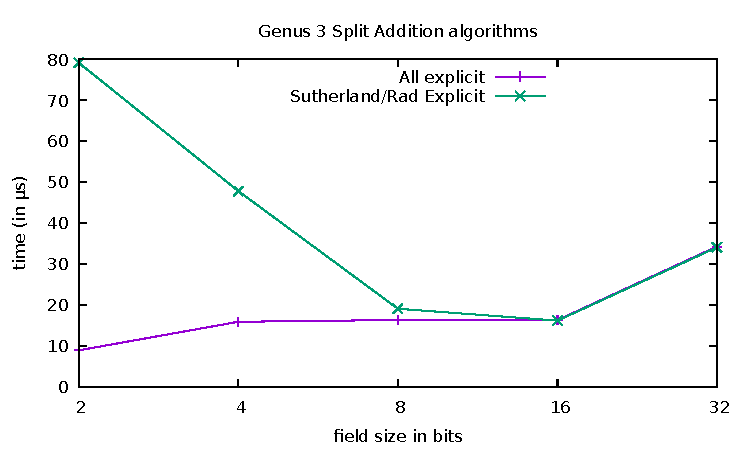
\includegraphics[width=0.775\textwidth]{genus3/g3_G1_ADD.pdf}}

\subsection{Split Model Comparisons}

In the next figures, explicit formulas introduced in this work are compared to
all relevant previous best algorithms over split models. The following
conclusions are drawn from these plots:
\begin{itemize}
    \item On the same platform, our explicit formulas outperform all relevant
    previous algorithms, including state-of-the-art and Cantor based algorithms
    for every field size.
     
    \item Our explicit formulas outperform Magma's built-in arithmetic over
    64-bit fields and up. Based on the relative performance of prior
    state-of-the-art, Magma is likely accessing internal $C$ functions that are
    not accessible via the interface provided.
\end{itemize}

\centerline{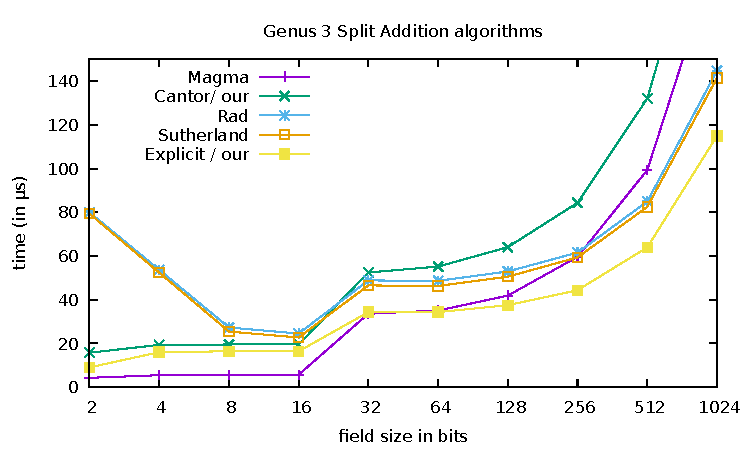
\includegraphics[width=0.775\textwidth]{genus3/g3_G2_ADD.pdf}}
\centerline{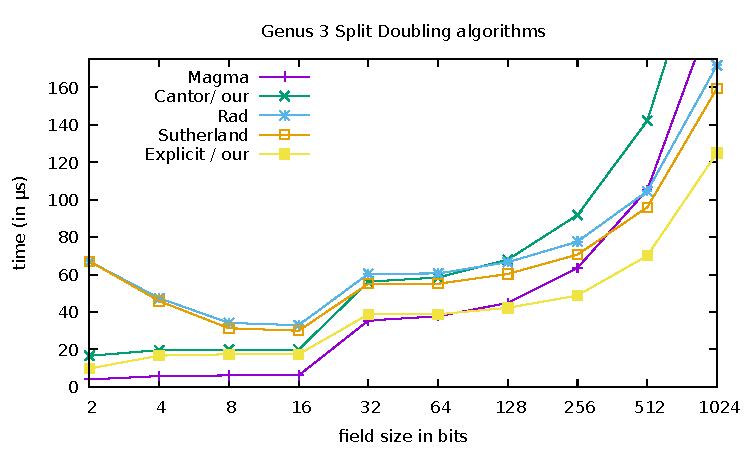
\includegraphics[width=0.775\textwidth]{genus3/g3_G2_DBL.pdf}}




The empirical results indicate that complete explicit formulas provide an
improvement for computing split model arithmetic over small
cardinality fields with a cross-over at 16-bits.  As expected, the relatively
fewer field operations (see Section~\ref{sec:g3comparisons}) in the formulas of
this work translate to faster implementations when using the same platform. The
relative performance of Magma's built-in arithmetic and the formulas of this
chapter likely due to Magma's high-level interface. Integrating algorithms from
this chapter directly into Magma's built-in arithmetic, or implementing the
algorithms directly in C/C++ so that they do not suffer from the overhead
associated to working in a high-level system like Magma, might reduce the
relative performance, and increase the field size for performance convergence
between complete explicit formulas and frequent case only implementations.